\documentclass{sig-alternate}
%\documentclass{vldb}
%\documentstyle{article}
%\documentstyle[amsmath,amsthm,amssymb,twocolumn]{article}
\usepackage{times}



\usepackage{MnSymbol} 
%\usepackage{MinionPro}
%\usepackage[mathlf,textlf,minionint]{MinionPro}
%\usepackage[T1]{fontenc}
%\usepackage{textcomp}
\usepackage{multirow}
%\usepackage{times}
\usepackage{pgfplots}
\usepackage{subfigure}
%\usepackage{amsmath,amssymb}
\usepackage{graphicx,color}
%\usepackage{verbatim}
%\usepackage{framed}
%\usepackage[ruled,vlined]{algorithm2e}

\usepackage[font={scriptsize,it}]{caption}
\usepackage{floatrow}


\begin{document}



\newcommand{\agp}[1]{\textcolor{red}{Aditya: #1}}
\newcommand{\mpv}[1]{\textcolor{blue}{Manasi: #1}}
%\newcommand{\alkis}[1]{\smallskip\noindent \textcolor{red}{\it $\Rightarrow$ Alkis: #1}}
\newcommand{\SeeDB}{{\sc SeeDB}}
\newcommand{\calQ}{\mathcal{Q}}
\newcommand{\calR}{\mathcal{R}}
\newcommand{\att}[1]{{\text{#1}}}

\newtheorem{definition}{Definition}[section]
\newtheorem{example}[definition]{Example}
\newtheorem{problem}{Problem}[section]
\renewcommand{\baselinestretch}{0.995}

%\DeclareMathOperator*{\argmax}{arg\!\max}




%\newcommand{\histvis}{\mbox{\sc HistVis}}
\newcommand{\squishlist}{
   \begin{list}{$\bullet$}
    { \setlength{\itemsep}{0pt}
      \setlength{\parsep}{2pt}
      \setlength{\topsep}{0pt}
      \setlength{\partopsep}{0pt}
      \leftmargin=25pt
\rightmargin=0pt
\labelsep=5pt
\labelwidth=10pt
\itemindent=0pt
\listparindent=0pt
\itemsep=\parsep
    }
}
\newcommand{\squishend}{\end{list}}

\newenvironment{denselist}{
    \begin{list}{\tiny{$\bullet$}}%
    {\setlength{\itemsep}{0ex} \setlength{\topsep}{0ex}
    \setlength{\parsep}{0pt} \setlength{\itemindent}{0pt}
    \setlength{\leftmargin}{0.5em}
    \setlength{\partopsep}{0pt}}}%
    {\end{list}}

\newcommand{\eat}[1]{}
\newcommand{\papertext}[1]{#1}
\newcommand{\techreport}[1]{}

\newcommand{\techreporttext}[1]{}
\newcommand{\stitle}[1]{\vspace{0.25em}\noindent\textbf{#1}}




\title{{\LARGE \sc SeeDB}: Automatically Generating Query Visualizations}
%\subtitle{\vspace{-10pt}[Vision Paper]\vspace{5pt}}



%\numberofauthors{3}
%\author{
%}

\maketitle
\begin{abstract}
%!TEX root=demo-paper.tex


% Data scientists rely on visualizations to interpret the data returned by
% queries, but finding the right visualization remains a manual task that is often
% laborious. We propose a DBMS that partially automates the task of finding the
% right visualizations for a query. In a nutshell, given an input query Q, the new
% DBMS optimizer will explore not only the space of physical plans for Q, but also
% the space of possible visualizations for the results of Q. The output will
% comprise a recommendation of potentially ``interesting'' or ``useful''
% visualizations, where each visualization is coupled with a suitable query
% execution plan. We discuss the technical challenges in building this system and
% outline an agenda for future research.
% 
Data analysts operating on large volumes of data 
often rely on visualizations to interpret the results of queries. 
However, finding the right visualization for a query is 
a laborious and time-consuming task. 
We demonstrate \VizRecDB, a system that partially automates 
this task: 
given a query, \VizRecDB\ explores the space of all possible visualizations,
and automatically identifies and recommends to the analyst those visualizations
it finds to be most ``interesting'' or ``useful''.
In our demonstration, conference attendees
will see \VizRecDB\ in action for a variety of queries on multiple real-world
datasets.





\end{abstract}
%% This is an example first chapter.  You should put chapter/appendix that you
%% write into a separate file, and add a line \include{yourfilename} to
%% main.tex, where `yourfilename.tex' is the name of the chapter/appendix file.
%% You can process specific files by typing their names in at the 
%% \files=
%% prompt when you run the file main.tex through LaTeX.
\chapter{Introduction}
\label{sec:introduction}

This thesis presents the design and implementation of a system, \SeeDB,
for automatically generating a large number of {\it interesting visualizations}
for any given query. There are two key challenges in automatically generating
visualizations: 1) automatically determining ``interesting''-ness of a
visualization, and 2) evaluating a large number of possible visualizations
efficiently.
In this work, we present solutions to both these problems.

\section{The data analysis process}
Data analysts must sift through very large volumes of data 
to identify trends, insights, or anomalies. 
Given the scale of data, and the relative ease and 
intuitiveness of examining data visually,
analysts often use visualizations as a tool to identify
these trends, insights, and anomalies.
However, selecting the ``right'' visualization often 
remains a laborious and time-consuming task. We illustrate the data analysis
process and challenges in choosing good visualizations using a few examples.

\subsection{Example 1: Business Intelligence}
Consider a dataset containing sales records for a nation-wide
chain of stores.
Let's say the store's data analyst is interested
in examining how the newly-introduced heating device, the ``Laserwave
Oven'', has been doing over the past year.
The results of this analysis will inform business decisions
for the chain, including marketing strategies, and the introduction of a similar
``Saberwave Oven''.

The analysis workflow proceeds as follows:
(1) The analyst poses a query to select the subset of data that she is
interested in exploring.
For instance, for the example above, she may issue the query:
\noindent $${\tt \ Q \ \ = \ \ SELECT \ * \ FROM \ \  Sales \ \ WHERE \ \
Product=``Laserwave''} $$ \noindent Notice that the results for this query may
have (say) several million records each with several dozen attributes.
Thus, directly perusing the query result is simply infeasible.
(2) Next, the analyst studies various properties of the selected data by
constructing diverse views or visualizations from the data. In this particular
scenario, the analyst may want to study total sales by store, quantity in stock
by region, or average profits by month. To construct these views, the analyst
can use operations such as binning, grouping, and aggregation, and then generate
visualizations from the view. For example, to generate the view `total sales by
store', the analyst would group each sales record based on the store where the
sale took place and sum up the sale amounts per store. This operation can easily
be expressed as the familiar aggregation over group-by query:
\noindent
\begin{align*}
& \tt Q' = SELECT \ \ store,\ SUM(amount) \ \ FROM \ \  Sales \ \ WHERE \\
& \tt Product=``Laserwave" \ \ GROUP  \ \ BY \ \ store
\end{align*}
The result of the above query is a two-column table that can then be visualized
as a bar-chart. Table \ref{tab:staplerX} and Figure
\ref{fig:staplerX} respectively show an example of the results of this view and
the associated visualization.

\begin{figure}[htb]

  \centering
    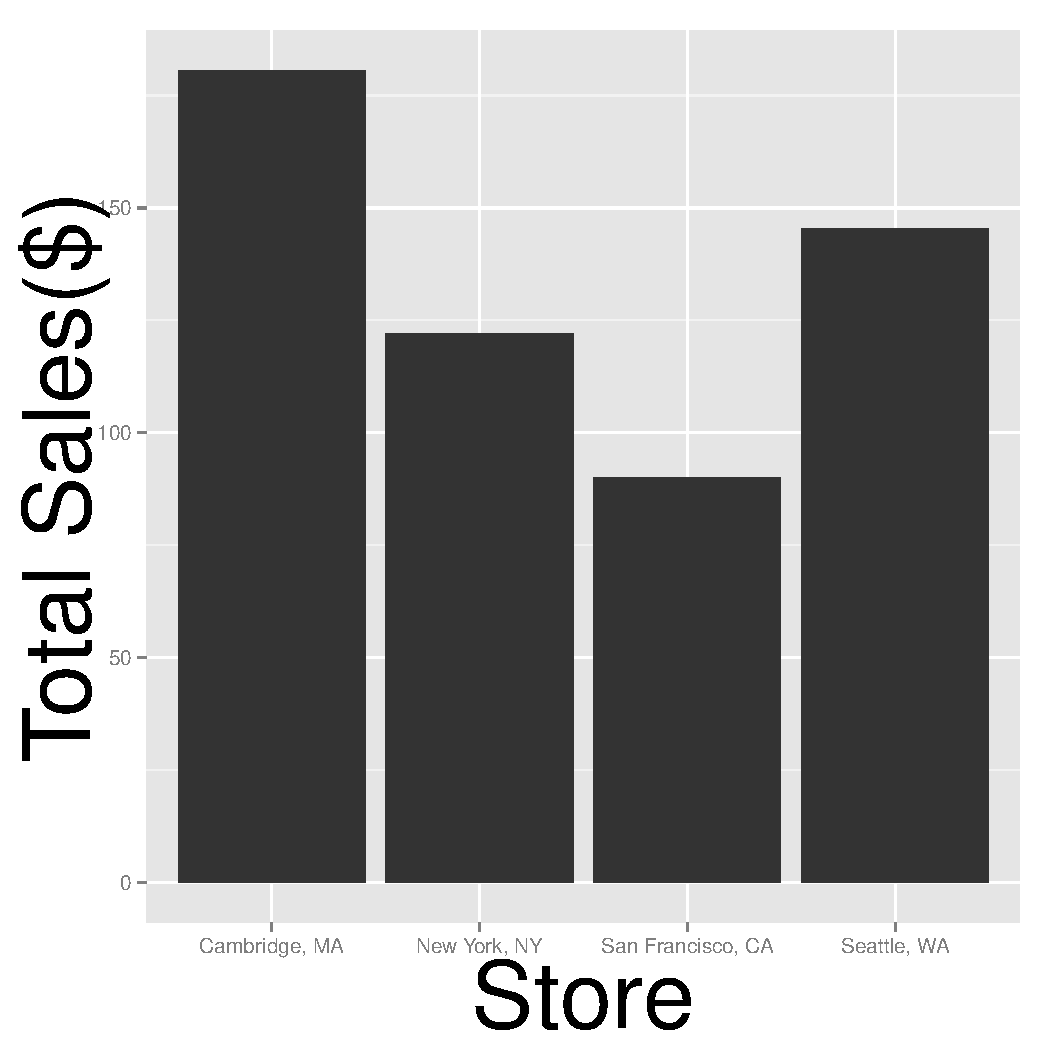
\includegraphics[width=12cm]{Images/dist1.pdf}
  \caption{Data: Total Sales by Store for Laserwave}
  \label{fig:staplerX}
\end{figure}

\begin{table}[htb]
  \centering
  \begin{tabular}{cc} \hline
  Store & Total Sales (\$) \\ \hline
  Cambridge, MA & 180.55 \\ \hline
  Seattle, WA &  145.50\\ \hline
  New York, NY & 122.00 \\ \hline
  San Francisco, CA & 90.13 \\ \hline
  \end{tabular}
  \caption{Data: Total Sales by Store for Laserwave}\label{tab:staplerX} 
\end{table}

\begin{figure}[htb]
  \centering
    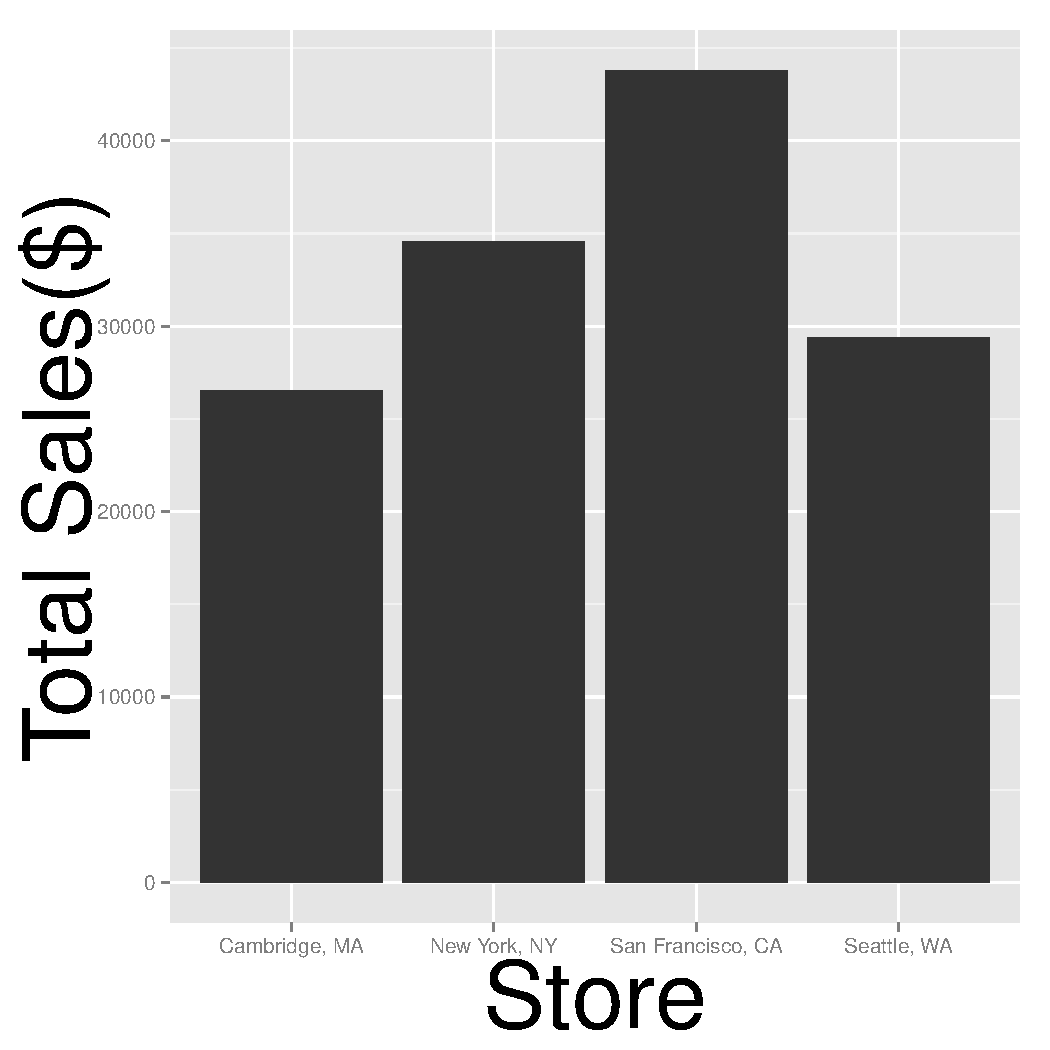
\includegraphics[width=12cm]{Images/dist2.pdf}
\caption{Scenario A: Total Sales by Store}
\label{fig:staplerX-a}
\end{figure}

\begin{figure}[htb]
  \centering
    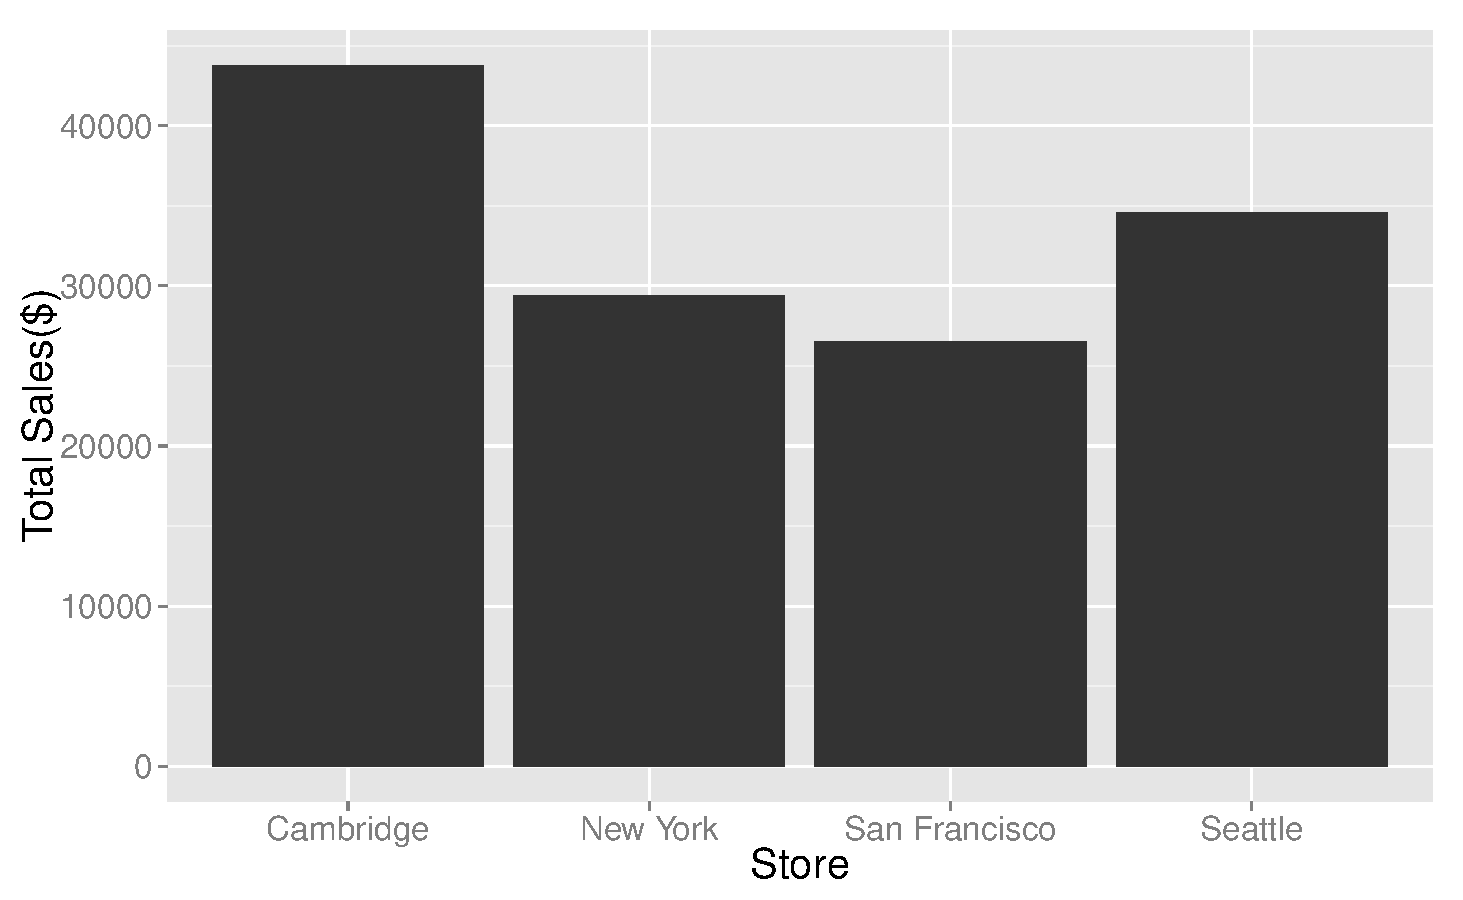
\includegraphics[width=12cm]{Images/dist3.pdf}
  \caption{Scenario B: Total Sales by Store}
  \label{fig:staplerX-b}
\end{figure}

To explore the query results from different perspectives, the analyst generates
a large number of views (and visualizations) of the form described above.
(3) The analyst then manually examines each view and decides
which ones are ``interesting''. This is a critical and time-consuming step.
Naturally, what makes a view interesting depends on the 
application semantics and the trend we are comparing against.
For instance, the view of Laserwave sales by store, as shown in Figure
\ref{fig:staplerX}, may be interesting if the overall sales of all products show
the {\it opposite} trend (e.g. Figure \ref{fig:staplerX-a}). However, the same
view may be uninteresting if the sales of all products follow a similar trend (Figure \ref{fig:staplerX-b}).
Thus, we posit that  a view is {\em potentially ``interesting'' if it shows 
a trend in the subset of data selected by the analyst
(i.e., Laserwave product-related data)
that deviates from the equivalent trend in the overall dataset}.
Of course, the analyst must decide if this deviation 
is truly an insight for this application.
(4) Once the analyst has identified interesting views, the analyst may
then either share these views with others, further interact with
the displayed views (e.g., by drilling down or rolling up), or
start afresh with a new query.


Of the four steps in the workflow described above, the 
ones that are especially repetitive and tedious are steps (2) and (3),
where the analyst generates a large number of candidate views, and examines each
of them in turn. The goal of our system, \SeeDB, is to automate these
labor-intensive steps of the workflow. Given a query $Q$ indicating the subset
of data that the analyst is interested in, \SeeDB\ automatically {\em identifies and highlights to the analyst the most
interesting views of the query results using methods based on
deviation}. Specifically, \SeeDB\ explores the space of all possible views and
measures how much each view deviates from the corresponding view on the
entire underlying dataset (e.g. Figure~\ref{fig:staplerX} vs.
Figures~\ref{fig:staplerX-a} or \ref{fig:staplerX-b}.) By generating and
scoring potential views automatically, \SeeDB\ effectively eliminates
steps (2) and (3) that the analyst currently performs. Instead, once \SeeDB\
recommends interesting views, the analyst can evaluate this small
subset of views using domain knowledge and limit further
exploration to these views.  

\subsection{Example 2: Medical Data}
Next, let us examine a use case in a completely different problem domain that
also involves analyses similar to Example 1, and therefore, can benefit from the
automatic construction of interesting views of a user query.

Consider a medical researcher studying the cost of care for cancer
patients\footnote{Real use scenario at an area hospital}. The goal of the study
is to identify patients whose cost of care is significantly greater than
average and try to explain the high cost of care. Potential reasons for
high cost include treatments for late-stage cancers, old age of the
population, longer survival time (chemotherapy for a longer duration), type of
treatment etc.
Note that the goal is {\it not} to build a predictive model for cost; rather, it
is to perform exploratory analysis to explain {\it why} certain patients have
high cost of care.
As a first pass, assume that the researcher identifies high cost patients as those with
cost that is greater than two standard deviations away from the average
cost. This can be expressed via the following SQL query, assuming a table of
patients with their treatment costs and other treatment-related information.
\begin{align*}
& \tt Q2\ = SELECT \ \ *\ FROM \ \ Patients \ \ where\ cost - \\
  \ \ & \tt (SELECT\ AVG(cost)\ FROM\ Patients)\ >\\
  \ \ & \tt 2\ *\ (SELECT\ STDDEV(cost)\ FROM\ Patients)
\end{align*}

Once these patients have been identified, the researcher can begin to analyze
the data to find potential reasons for their high cost of care (This is similar
to Step 1 in Example 1).
One technique to find potential reasons for high cost is to compare the
high-cost population of patients to the remaining set of patients (called
``low-cost'' population).
Similar to Example 1 above, we posit that the {\it characteristics that
explain high cost are precisely those characteristics that are different between
the high-cost and low-cost population}. 
For instance, if the majority of
high-cost patients were those with late-stage disease (sicker patients) while
the low-cost patients were not, the researcher could reason that the sicker
patients needed more medications or procedures, leading
to higher cost overall. 
Note that this analysis is similar to Example 1 where we
compared the ``total sales by year'' for $Laserwave$ $oven$ vs. all store
products.
In this setup, we want to compare the ``total patients by disease stage'' for
high-cost patients vs. low-cost patients. The only change in the problem
formulation is that we are now comparing views of query Q2 against views of the
remaining table, instead of views over the entire table. The rest of the
framework remains unchanged. Therefore, \SeeDB\ can be used to automatically
construct a large number of views of the high-cost population, compare
each view to the corresponding view over the low-cost population, and
identify views showing the highest difference between the two populations. These
views identify potential causes for high cost. Once the researcher has identified views of interest, he or she
can follow up with more complex analyses like statistical significance testing or machine
learning.

\subsection{Example 3: Product Analysis}

Consider a company like Facebook\footnote{www.facebook.com} that continuously
deploys changes to its website and mobile apps, and tracks user interaction
through detailed logging. Product specialists at Facebook use these logs to
study how different Facebook users respond to changes to the web or mobile
experience \cite{DBLP:conf/vldb/AbrahamABB13}. Each user can be characterized by a large number
of features such as location, age, device used, number of friends etc.
For each user, the logs note the actions taken on the website or app such
as likes, shares, comments, page visits etc. For example, in order to study
the user response to an update to the mobile app, the specialist compares user
interaction metrics for a large number of mobile users before and after the
update (usually a week on week comparison). The goal is to find patterns in the
interaction metrics based on different user characteristics. Therefore, if it
appears that the average number of app visits on the iOS app have reduced
signficantly following the update, it would indicate a problem with the iOS app.

In terms of the \SeeDB\ framework, log data from the week following the app
update constitutes the query results we seek to analyze and the log data from
the prior week comprises the comparison dataset. As in Examples 1 and 2, the
analysis process requires the specialist to create diverse views of the query
results, compare views to equivalent views on the comparison dataset, and
pick the views showing the highest difference. 
\SeeDB\ can therefore be used to automate this process and surface only the most
interesting views.

\subsection{\SeeDB}
This thesis describes a prototype of the \SeeDB\ system that finds interesting
visualizations of query results. 
Given a query $Q$ indicating the subset of data that the analyst is interested in, \SeeDB\ automatically {\em identifies and highlights to the
analyst the most interesting views of the query results using methods based on
deviation}. 
Our prototype is based on
\cite{DBLP:conf/vldb/Parameswaran2013} which describes the vision for \SeeDB.

To efficiently and accurately identify interesting views of any given query, we
are faced with the following challenges:
\begin{itemize}
  \item We must determine metrics that accurately measure the ``deviation'' of a
view with respect to the equivalent view on the entire database (e.g.,
Figure~\ref{fig:staplerX} vs.~\ref{fig:staplerX-a}), while simultaneouly
ensuring that \SeeDB\ is not tied to any particular metric(s)
\item We must
intelligently explore the space of candidate views. Since the number of
candidate views (or visualizations) increases as the square of the number of
attributes in a table (we will demonstrate this in subsequent sections),
generating and evaluating all views, even for a moderately sized dataset (e.g.
1M rows, 100 attributes), can be prohibitively expensive
\item While executing
queries corresponding to different views, we must share computation as much as
possible. For example, we can compute multiple views and measure their deviation
all together in one query. Independent execution, on the other hand, will be
expensive and wasteful
\item Since analysis must happen in real-time, we must trade-off accuracy of
visualizations or estimation of ``interestingness'' for reduced latency.
\end{itemize}

Contributions of the work described in this thesis are:
\begin{itemize}
  \item We implement the \SeeDB\ system based on \cite{DBLP:conf/vldb/Parameswaran2013} to
  automatically find interesting views of queries (Chapter
  \ref{sec:system_architecture}).
  \item We propose and implement a number of optimizations to
  efficiently perform the search for interesting views and share
  computation between multiple views simultaneously (Chapter
  \ref{sec:optimizations}).
  \item We evaluate the performance of our optimizations on a range of datasets
  and demonstrate the resulting 100x speedup (Chapter
  \ref{sec:experiments}).
  \item We model the performance of \SeeDB\ in terms of various parameters of
  \SeeDB\ and the underlying database, and use this model to identify optimal
  parameter settings for \SeeDB\ (Chapter \ref{sec:model}).
  %\item We present and evaluate different metrics for measuring deviation
  %\item ?? We study the usefulness of a tool like \SeeDB\ in finding
  %interesting visualizations of a dataset
\end{itemize}



% of Step 1), we demonstrate that we can automatically explore various views of
% that data, evaluate each one for ``interesting''-ness and only surface the most
% promising views to the analyst. 



% In this demo, we demonstrate a system called \SeeDB\
% \cite{DBLP:conf/vldb/Parameswaran2013} that automates the labor-intensive parts
% of the aforementioned data analysis process by automatically identifying and
% producing high-quality views for any input query. Specifically, given a query
% $Q$ posed by the user, \SeeDB\ explores all possible views of $Q$, determines
% the ``interesting''-ness of each of the views based on deviation and returns to
% the user the set of views that it deems the most interesting. The user can then
% limit his analysis to this high-quality set of views.

% In the process of automatically producing an interesting set of views for any
% query, \SeeDB\ must address a few challenges: (a) the size of the space of
% potential views increases as the square of the number of attributes in a table,
% and even for a moderately sized table (e.g. 1M rows, 100 attributes) generating
% all views is prohibitively expensive; as a result, \SeeDB\ must intelligently
% explore this space; (b) computing each view and its utility independently is
% expensive and wasteful, and hence \SeeDB\ must share computation between
% queries; and (c) since visual analysis must happen in real-time, \SeeDB\ must
% tradeoff accuracy of views for reduced latency. In Section
% \ref{sec:system_architecture}, we describe how \SeeDB\ addresses these
% challenges.


% Consider a medical researcher studying the cost of care for cancer patients. Her
% research involves the analysis of a set of 1M electronic medical records (EMRs).
% To analyze this data, the researcher identifies patients that cost
% significantly more than the average: specifically, she selects patients whose
% cost of care is greater than the average cost by two standard deviations. In
% terms of SQL, she runs the following query: \\

% \noindent 
% \begin{small}
% \begin{verbatim}
% Q = SELECT * FROM Patients where total_cost - 
% (SELECT AVG(total_cost) from Patients) as avg_cost
% > 2 * (SELECT STDDEV(total_cost) from Patients);
% \end{verbatim}
% \end{small}

% Once she has identified these patients, she must study various aspects of their
% care to determine the reason why the patients have large cost of care. For
% instance, she may study length of treatment, survival rate, severity of disease
% etc. For each of these parameters, she is interested in determining how the
% group of patients with high cost of care are different from the overall group of
% patients. As a result, she may construct various views of the data that
% compare various metrics between the high cost patients and the overall patient
% population. For instance, she may compare the distribution of length of
% treatment for the two populations, the average severity of the disease
% etc. Since there are a large number of metrics that may be responsible for high
% cost of care, the analyst must construct, visualize and examine a large number
% of views to identify interesting trends. For more than 5 metrics, this process
% quickly becomes tedious and time-consuming. We can significantly simplify and
% speed up the analysis process if we can automate the creation and evaluation of
% views.


% \begin{figure}
% \vspace{-10pt}
% \CenterFloatBoxes
% \begin{floatrow}
% \ttabbox{%
%   \small
%   \begin{tabular}{cc} \hline
%   Store & Total Sales (\$) \\ \hline
%   Cambridge, MA & 180.55 \\ \hline
%   Seattle, WA &  145.50\\ \hline
%   New York, NY & 122.00 \\ \hline
%   San Francisco, CA & 90.13 \\ \hline
%   \end{tabular}
% }{%
%   \caption{Data: Total Sales by Store for Laserwave}\label{tab:staplerX}%
% }
% \killfloatstyle
% \ffigbox{%
%   \hbox{\resizebox{2cm}{2cm}{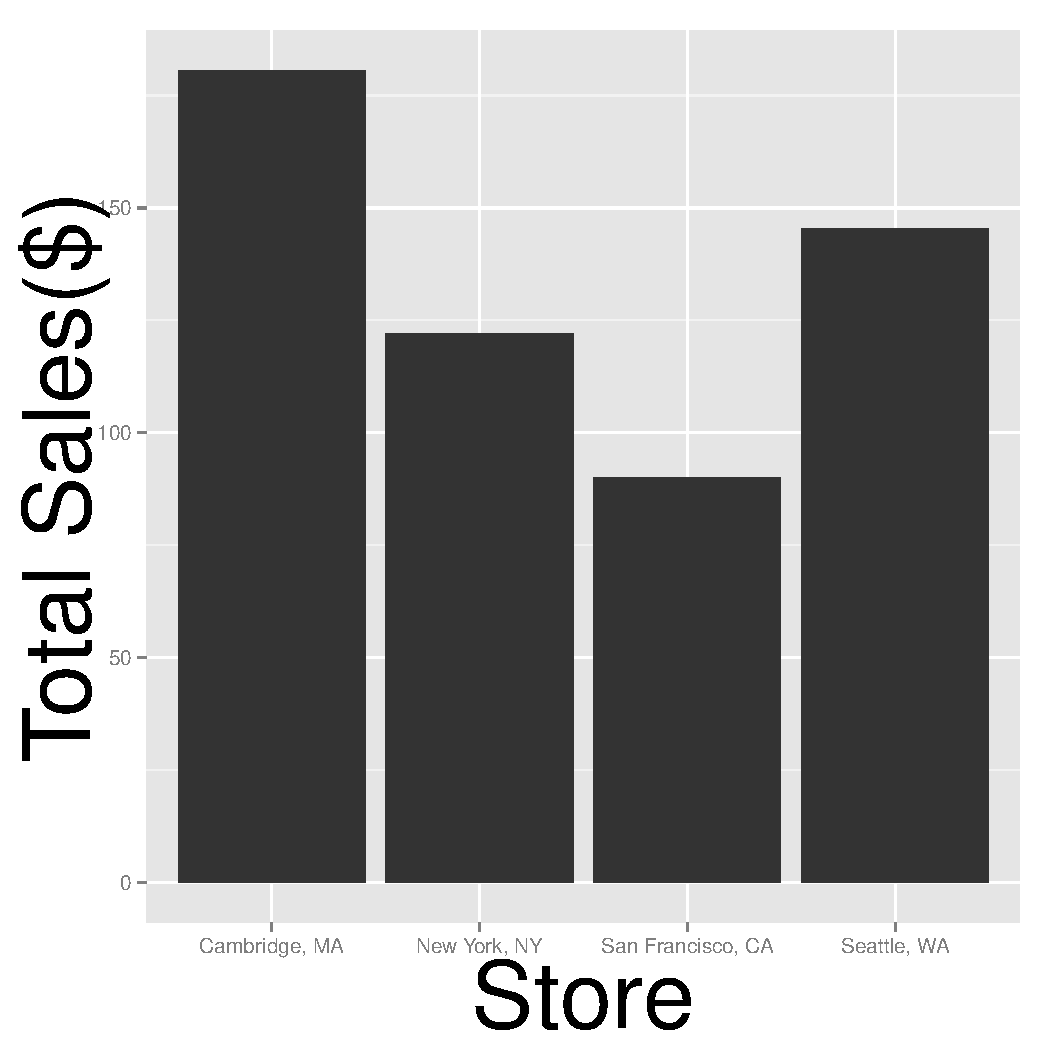
\includegraphics{Images/dist1.pdf}}}
%   
% }{%
%   \caption{Visualization: Total \\ Sales by Store for
%   Laserwave}
%   \label{fig:staplerX}%
% }
% \end{floatrow}
% \end{figure} 
%  
% \begin{figure}
% \CenterFloatBoxes
% \begin{floatrow}
% \centering
% \ffigbox{%
%   \hbox{\resizebox{2cm}{2cm}{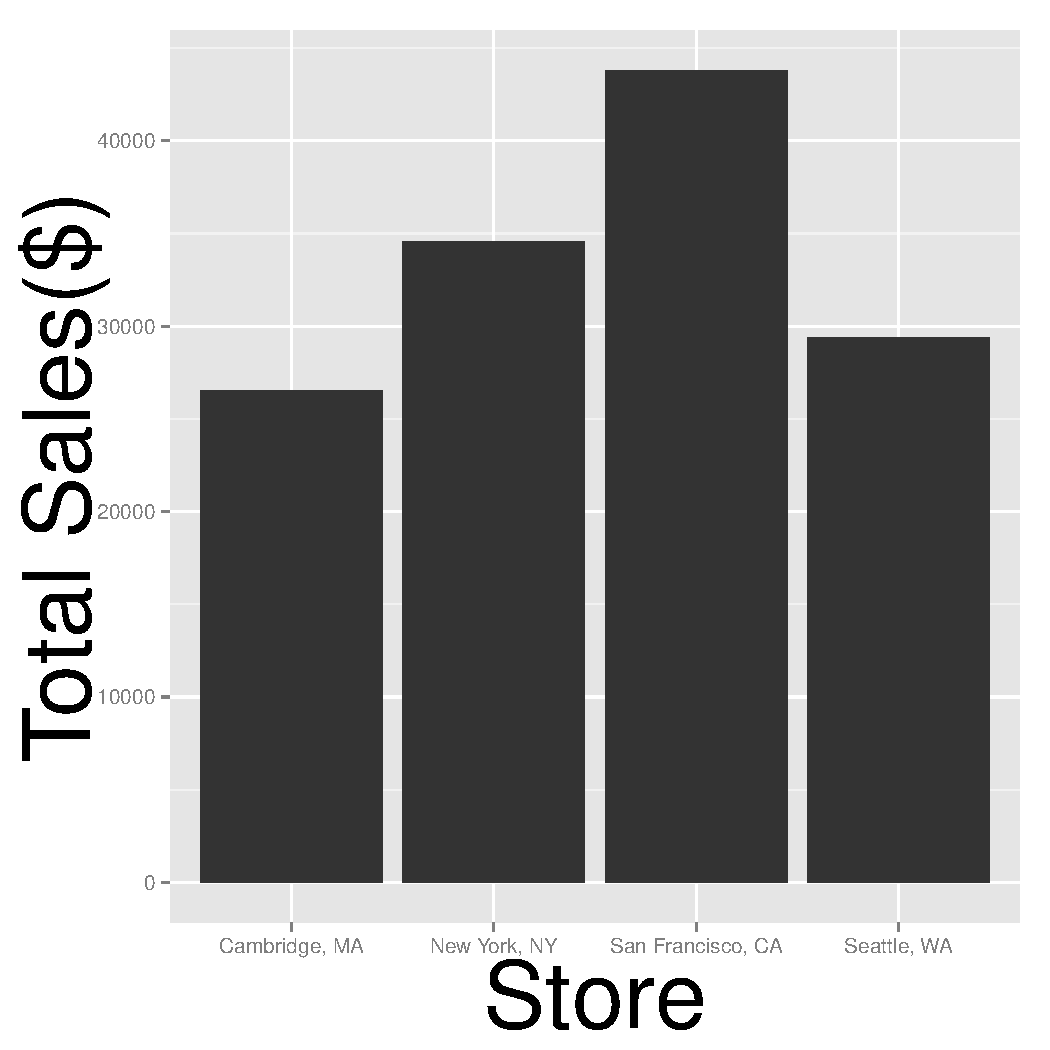
\includegraphics{Images/dist2.pdf}}}
% 
% }{ \caption{Scenario A: Total Sales by Store}\label{fig:staplerX-a}%
% }
% \killfloatstyle
% \ffigbox{%
%   \hbox{\resizebox{2cm}{2cm}{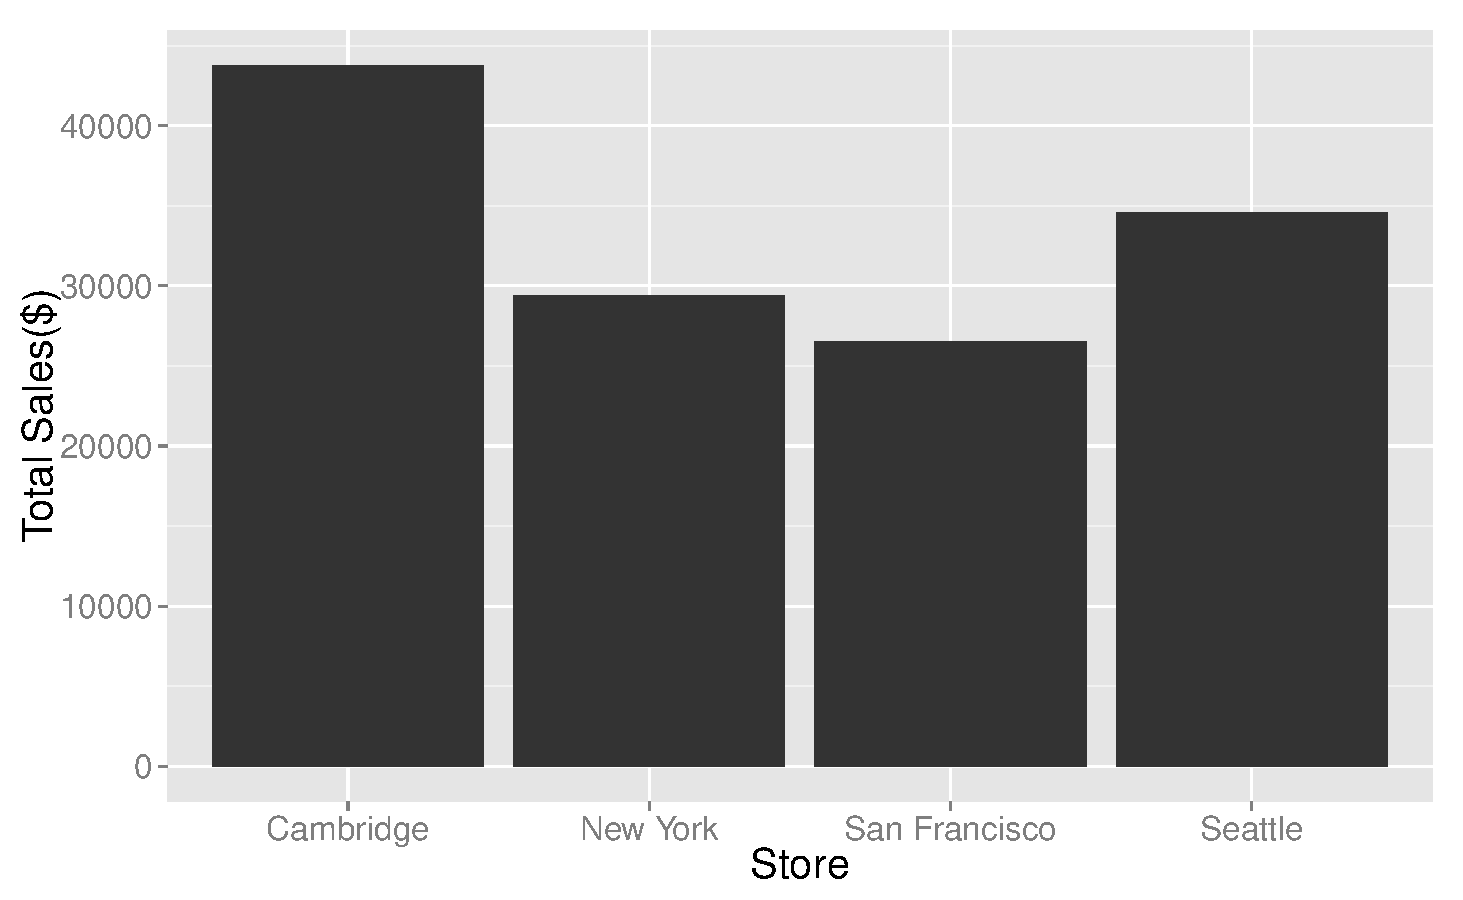
\includegraphics{Images/dist3.pdf}}} 
% 
%   }{\caption{Scenario B: Total Sales by Store}
%   \label{fig:staplerX-b}%
%   }
% \end{floatrow}
% \vspace{-12pt}
% \end{figure}


% Since \SeeDB\ must rank views based on utility, accurately measuring 
% utility is cruicial. \SeeDB\ is based on the principle
% that it is the {\bf deviations from expected behavior that make a view
% interesting}. For instance, in the above example, the researcher would be
% interested in the fact that high-cost patients actually visit a specific set of
% doctors compared to the entire patient population. Similarly, the researcher
% would be interested in knowing that the high-cost patients have longer hospital
% stays compared to the rest of the population. Thus, given a query, interesting
% trends are those that differ significantly between the query and the underlying
% dataset. \SeeDB\ therefore assigns higher utility to views that show divergent
% trends. (Since it may be more appropriate to compare the high-cost patients with
% other patients having the same disease but lower cost, so \SeeDB\ allows the
% user to specify what dataset to compare with).


% \noindent There are several technical challenges that need to be addressed:
% 
% \begin{denselist}
% 
% \item For a given query, $n$, the total number of discriminating views, (even if
% we restrict ourselves to views that append a group-by and an aggregation) is
% likely to be very large to explore exhaustively and precisely. Generating each
% of $R_1(Q(D)),$  $\ldots,$ $R_n(Q(D))$, scoring them on utility, and then
% picking the best one is certainly not feasible for most databases. Thus, we need
% mechanisms to prune the space of views and compute their utility approximately.
% 
% \item Generating and scoring the discriminating views $R_i(Q(D))$ one-by-one may
% miss interesting optimization opportunities: First, we may share computation
% between discriminating views.  For example, the results of two views with
% different aggregates but the same group-by may be computed together in one
% query, followed by projecting out to reveal the two individual views.  Second,
% by evaluating the discriminating views in a deliberate order, we may be able to
% prune views with low utility (without evaluation) that are definitely not going
% to be recommended to the analyst.
% 
% \item Since visualizations tend to convey approximate information, e.g., a trend
% in a line plot may be more important than knowing the exact coordinates of each
% point, we can introduce approximations as part of \SeeDB.  Thus, the utility of
% a discriminating view may be computed approximately but efficiently, and the
% recommended discriminating views can be populated with approximate results,
% based on synopses of the base data or of the query result, that can be generated
% much more efficiently.
% 
% \end{denselist}

%!TEX root=demo-paper.tex


\section{Problem Statement}
\label{sec:problem_statement}

Given a database $D$ and a query $Q$, \SeeDB\ considers a number of views that
can be generated from $Q$ by adding relational operators.
For the purposes of this discussion, we will refer to views and visualizations
interchangeably, since it is straightforward to translate views into
visualizations automatically. For example, there are straightforward rules that
dictate how the view in Table~\ref{tab:staplerX} can be transformed to give a
visualization like Figure~\ref{fig:staplerX}.
Furthermore, we limit the set of candidate views to those
that generate a two-column result via a single-attribute grouping and
aggregation (e.g. Table~\ref{tab:staplerX}). However, \SeeDB\ techniques can
directly be used to recommend visualizations for
multiple column views ($> 2$ columns) that are generated via multi-attribute
grouping and aggregation.

%Lastly, for simplicity, 
%we ignore {\em binning}: that is, given a view to be visualized,
%there are many ways of binning values to give the view. 
%For instance, if we have average profits per day, we can bin the days into
%months, into weeks, or into years.

We consider a database $D$ with a snowflake schema,
with dimension attributes $A$, measure attributes $M$, and potential
aggregate functions $F$ over the measure attributes.
We limit the class of queries $Q$ posed over $D$ to be
those that select one or more rows from the fact table, and denote the results
as $D_Q$. 
%select a horizontal fragment of the fact table:
%this selection can be done using selection predicates on the fact
%table, or on dimension tables via key-foreign-key joins.
%Overall, this class of queries allows the analyst to express their interest
%in examining facts (i.e., a slice of the dataset)
%that satisfy specific conditions.
%We denote the result of $Q(D)$ as $D_Q$.

Given such a query $Q$, \SeeDB\ considers all views $V_i$ that perform a
single-attribute group-by and aggregation on $D_Q$. We represent $V_i$ as a
triple $(a, m, f)$, where $m \in M, a \in A, f \in F$, i.e., the view
performs a group-by on $a$ and applies the aggregation function $f$ on a measure
attribute $m$. We call this the {\em target view}.
%Thus, $V_i (D_Q)$ can be expressed as the following SQL query:
$${\tt SELECT \ } a, f(m) \ \ {\tt FROM} \  D_Q\  {\tt GROUP \ \ BY} \ a$$ 
As discussed in the previous section, \SeeDB\ evaluates
whether a view $V_i$ is interesting
by computing the deviation between the view applied to the selected data (i.e., $D_Q$) 
and the view applied to the entire database.
The equivalent view on the entire database $V_i (D)$ can be expressed as shown
below that we call the {\em comparison view}. 
$${\tt SELECT \ } a, f(m) \ \ {\tt FROM} \  D\  {\tt GROUP \ \ BY} \ a$$
The results of both the above views are tables with two columns, namely $a$ and
$f(m)$. We normalize each result table into a probability distribution, such
that the values of $f(m)$ sum to $1$.
% over the various values of $a$ and the tables can be normalized into
%probability distributions for comparison. To convert each result table 
For our example in Table~\ref{tab:staplerX}, the probability distribution of
$V_i(D_Q)$, denoted as $P[V_i (D_Q)]$, is: (Jan: 180.55/538.18, Feb:
145.50/538.18, March: 122.00/538.18,  April: 90.13/538.18). A similar
probability distribution can be derived for $P[V_i (D)]$.

Given a view $V_i$ and probability distributions for the
target view  ($P[V_i (D_Q)]$) and comparison view ($P[V_i (D)]$), the
{\em utility} of $V_i$ is defined as the distance between these two probability
distributions. Formally, if $S$ is a distance function,
$$ U (V_i) = S ( P[V_i (D_Q)], P[V_i (D)] )$$

The utility of a view is our measure for whether the target view is
``potentially interesting'' as compared to the comparison view:
the higher the utility, the more the deviation
from the comparison view, and the more likely the view is to be interesting.
Computing distance between probability distributions has
been well studied, and \SeeDB\ supports a variety of metrics
to compute utility, including Earth Movers Distance, 
Euclidean Distance, Kullback-Leibler (K-L) Divergence, and Jenson-Shannon
Distance. 

Finally, we note that while other definitions of the comparison views and
utility metrics are possible, for our initial exploration into 
visualization recommendations, we chose to focus on the intuitive definitions above.

\begin{problem}
\vspace{-5pt}
Given an analyst-specified query $Q$ on a database $D$, a distance function $S$,
and a positive integer $k$, find $k$ views $V \equiv (a, m, f)$ that
have the largest values of $U(V)$ among all the views that can be represented
using a triple $(a, m, f)$, while minimizing total computation time.
\vspace{-5pt}
\end{problem}

Thus, \SeeDB\ aims to find the $k$ views (obtained by adding a single aggregate
and group-by operator) that have the largest utility based on the function $U$.



\subsection{Extensions}
There are two important variations of the problem that can be addressed exactly
by the same techniques discussed in the paper. These are:

\vspace{5 mm}

\squishlist
\item {\bf Group-by clauses with multiple dimension attributes}: It is
straightforward to extend the \SeeDB\ techniques  to group-by clauses with multiple attributes.
However, for ease of exposition and visualization, we limit the number of
attributes in the group-by clause to one.
\item {\bf Comparison of two-queries}: Instead of comparing the views of
the input query to the entire underlying dataset, it may be more appropriate to
compare them to another subset of the data (e.g. sales of ``Staplers'' vs.
sales of ``Printers''). This simply involves replacing the dataset parameter $D$
with a second query $Q'$. This variation is important since it can help users
find interesting differences in data. Our techniques apply to this variation
unchanged and we show experimental results for this variation.
\squishend


%Trend in the subset of the data that deviates from the corresponding trend in
%the overall data.
\section{State-of-the-Art Approaches}
\label{sec:related_work}

Over the past few years, there has been a significant
effort from the visualization community to provide interactive tools
for data analysts. In particular, tools such as ShowMe, Polaris, and
Tableau~\cite{DBLP:journals/cacm/StolteTH08,
  DBLP:journals/tvcg/MackinlayHS07} provide a canvas for data analysts
to manipulate and view data, tools such as
Wrangler~\cite{DBLP:conf/chi/KandelPHH11} allow data analysts to
transform and clean data, and tools such as
Profiler~\cite{DBLP:conf/avi/KandelPPHH12} allow users to visualize
simple anomalies in data.  However, unlike \SeeDB, these tools have
little automation; in effect, it is up to the analyst to generate a
two-column view to be visualized. Other related areas of work include OLAP and
database visualization tools. There has been some work on browsing data cubes, allowing
analysts to variously find ``explanations'' for why two cube values were
different, to find which neighboring cubes have similar properties to the cube
under consideration, or get suggestions on what unexplored data cubes should be
looked at next~\cite{DBLP:conf/vldb/Sarawagi99, DBLP:conf/vldb/SatheS01,
DBLP:conf/vldb/Sarawagi00}.

Fusion tables~\cite{DBLP:conf/sigmod/GonzalezHJLMSSG10} allows users to create
visualizations layered on top of web databases; they do not consider the problem
of automatic visualization generation.
Devise~\cite{DBLP:conf/sigmod/LivnyRBCDLMW97} translated user-manipulated
visualizations into database queries.

\subsection{Viz papers and tools}
\subsection{Data Cubes}
\subsection{General ML and stats references}
\subsection{Multi-query optimization} 
\section{System architecure}
\label{sec:system_architecture}

In this section, we present the architecture of \SeeDB\ starting with an
overview, followed by a detailed discussion of the various modules in \SeeDB.

\subsection{\SeeDB\ architecture overiew}
\label{subsec:overview}

Our prototype of \SeeDB\ is designed as a layer on top of a relational database
system.
While optimization opportunities are restricted by virtue of being outside the
database, our design permits \SeeDB\ to be used in conjunction with a variety of
existing database systems. \SeeDB\ is comprised of two main parts: the \SeeDB\
front end and the \SeeDB\ backend. The front end is a ``thin client'' that
is only used to issue queries to \SeeDB\ and view results. The backend in
contrast performs all the computation required to generate and select views. Figure \ref{fig:sys-arch}
shows the architecture of our system.

\begin{figure}[htb]
\centerline{
\hbox{\resizebox{9cm}{!}{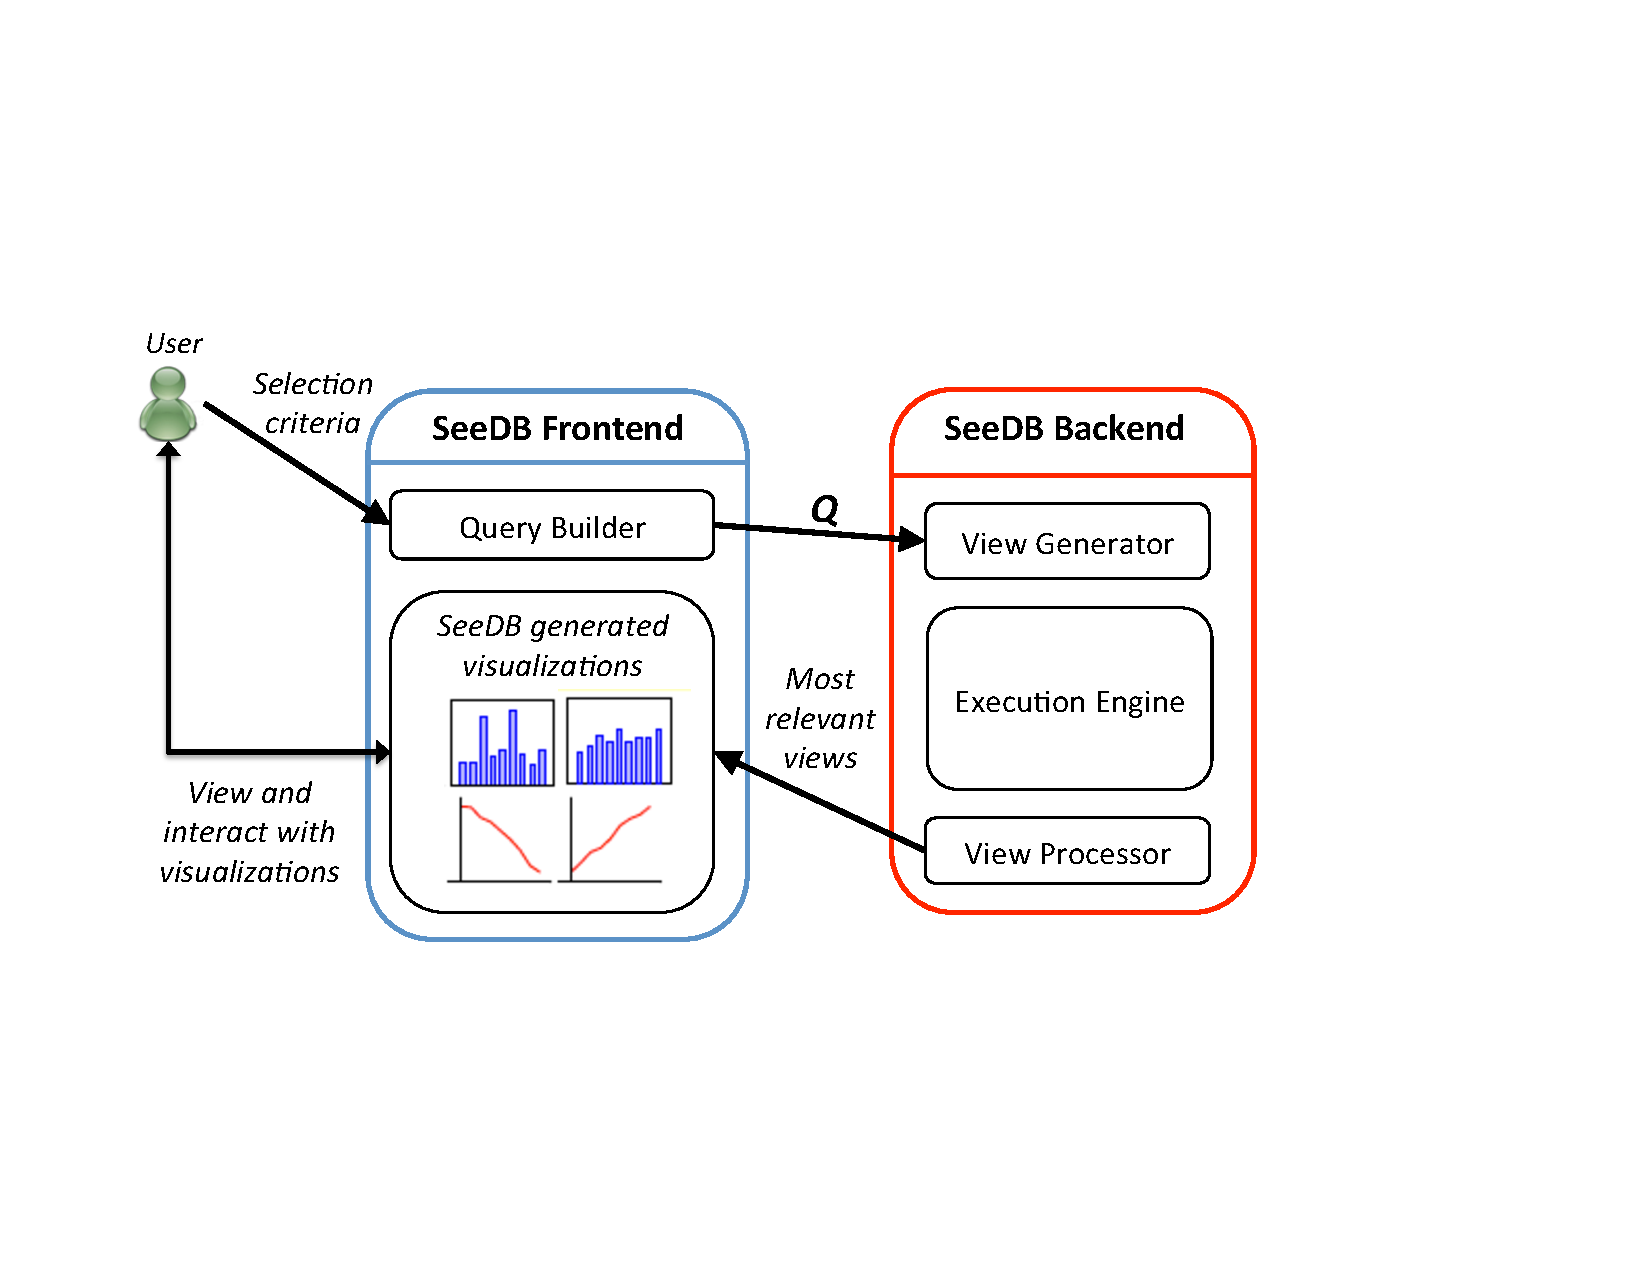
\includegraphics[trim=10mm 50mm 10mm 50mm,
clip=true]{Images/seedb-architecture.pdf}}}}
\caption{SeeDB Architecture}
\label{fig:sys-arch}
\end{figure} 

An analyst uses the front end to issue queries to \SeeDB. We provide three
mechanisms for the analyst to issue queries: raw SQL, an intuitive
query-builder, and a set of pre-formulated queries for common operations on a
dataset (we discuss query input further in Section \ref{subsec:seedb_frontend}).
Once the analyst issues a query via the \SeeDB\ front end, the backend
takes over.
First, the Metadata Collector module queries metadata tables (a combination of
database-provided and \SeeDB\ specific tables) for information such as table
sizes, column types, data distribution, and table access patterns.
The resulting metadata along with the analyst's query is then passed to the
Query Generator module. The purpose of the Query Generator is two-fold:
first, it uses the metadata obtained in the previous step to prune the space of
candidate views to the most promising ones; and second, it generates target and
comparison views for each view that has not been pruned.
The SQL queries corresponding to the target and comparison views are then passed
to the Optimizer module. We refer to these queries collectively as {\it view
queries}.
The Optimizer module is responsible for determining the best way to combine
view queries intelligently so that the total execution time is
minimized. 
(We discuss the optimizations performed by the Query Generator and
Optimizer modules further in Section \ref{subsec:seedb_backend}.) Once the
Optimizer module has generated the optimized queries, \SeeDB\ sends the
queries to the underlying database system for execution. The results returned by
the DBMS are then processed by the View Processor module. This module processes
results of the optimized queries in a streaming fashion and produces results for
individual views. Results of individual views are then normalized as discussed
in Section~\ref{sec:problem_statement} and the utility of each view is computed.
Finally \SeeDB\ selects the top $k$ views with the highest utility and returns them to the
\SeeDB\ front end. The \SeeDB\ frontend creates visualizations for each
view and displays the visualizations to the analyst.

We now discuss the major \SeeDB\ modules in detail.

\subsection{SeeDB Frontend}
\label{subsec:seedb_frontend}

The \SeeDB\ frontend, designed as a thin client, performs two main functions: it
allows the analyst to issue a query to \SeeDB, and it visualizes the results (views) produced by the \SeeDB\
backend.
To provide the analyst maximum flexibility in issuing queries, \SeeDB\
provides the analyst with three
mechanisms for specifying an input query: 
(a) writing raw SQL, (b) using a query builder that allows analysts
unfamiliar with SQL to formulate queries through a form-based interface, and (c)
using pre-defined query templates which encode commonly performed operations,
e.g., selecting outliers in a particular column. We find that pre-defined query
templates are particularly useful since analysts are often interested in
anomalous data points.

Once the analyst issues a query via the \SeeDB\ frontend, the \SeeDB\ backend
evaluates various views and sends the most interesting ones back to the
frontend.
For each view returned by the backend, the \SeeDB\ frontend determines the best
way to visualize the view depending on parameters such as the data
type (e.g. ordinal, numeric), number of distinct values and semantics (e.g.
geography vs.
time series).
The resulting set of visualizations is displayed to the analyst who can easily
examine these ``most interesting'' views at a glance, explore specific views in detail and
view metadata for each view (e.g. size of result, sample data, value with
maximum change and other statistics). 
The analyst can also slice-and-dice views further by performing drill-downs on
the relevant attributes in the view. 
Figure~\ref{} shows a screenshot of the \SeeDB\ frontend in action.
%This action automatically
%modifies the selection query and displays views for the subset of data
% selected. The user can of course revert back to the original views and continue exploring the data.

\subsection{SeeDB Backend}
\label{subsec:seedb_backend}

As discussed in Section \ref{subsec:overview}, \SeeDB\ is implemented using a
light-weight frontend described in the previous section and a backend that
performs all the computations for generating and selecting views. Furthermore,
as shown in Figure~\ref{fig:sys-arch}, the \SeeDB\ backend is composed of four
modules that are respectively responsible for collecting metadata (Metadata Collector), pruning
the view space and generating view queries (Query Generator), optimizing view
queries (Optimizer), and processing query results to identify the top-$k$
interesting views (View Processor). In this section, we will discuss the various
techniques underlying \SeeDB. To achieve its goal of finding the most
interesting views accurately and efficiently, \SeeDB\ must not only accurately
estimate the accuracy of a large number of views but also design ways in which
the total processing time will be minimized.
We first describe the basic \SeeDB\ framework and then briefly discuss our optimizations.

% One of the chief challenges in \SeeDB\ is producing the most interesting views
% of the query result in the least possible time. For achieve the above
% performance goal, \SeeDB\ must perform optimizations at two stages: first, using
% prior knowledge such as statistics to prune out uninteresting views without examining table data; and second, minimizing the
% execution time for queries that are issued to the database. 

\subsubsection{Basic Framework}
\label{subsubsec:basic_framework}

Given a user query $Q$, the basic technique used in \SeeDB\ computes all
possible views obtained by adding a single aggregate and a single group-by
clause to $Q$. Target and comparison views corresponding to each view are then
computed and each view query is executed independently on the DBMS. The query
results for each view are normalized to compute the target and comparison view
probability distributions. The utility of a given view is computed as the
distance between these two distributions (Section \ref{sec:problem_statement}).
Finally, the top-$k$ views with the largest utility are chosen. 

The basic approach is clearly inefficient
since it examines each possible view and executes each view query independently;
we next discuss how our optimizations fix some of these problems.

\subsubsection{View Space Pruning}
\label{subsubsec:view_space_pruning}

Most views possible for any query $Q$ have low utility since the target view
distribution is very similar to the comparison view distribution. 
As a result,
\SeeDB\ aggressively prunes view queries that are unlikely to have high
utility. 
This pruning is based on metadata about the table including data
distributions and access patterns.
We leverage table metadata in several ways, some of which are listed below:
\begin{denselist}
\item {\it Variance-based pruning}: Dimension attributes with low variance are
likely to produce views having low utility (e.g. consider the extreme case where
an attribute only takes a single value); as a result, \SeeDB\ prunes views
containing grouping attributes with low variance.
\item {\it Correlated columns}: If two dimension attributes $a_i$ and $a_j$ have
a high degree of correlation (e.g. full name of airport and abbreviated name of
airport), the views generated by grouping the table on $a_i$ and $a_j$ will be
very similar (and have almost equal utility). We can therefore generate and
evaluate a single view representing both $a_i$ and $a_j$. \SeeDB\ clusters
attributes based on correlation and evaluates a single representative view per
cluster.
\item {\it Access Frequency Pruning}: In tables with a large number of
attributes, only a small subset of attributes are relevant to the analyst and
are frequently accessed for data analysis. \SeeDB\ tracks access patterns
for each table to identify the most frequently accessed columns and combinations of
columns. While creating views, \SeeDB\ uses this information to prune attributes
that are rarely accessed and are thus likely to be unimportant.
\end{denselist}

\subsubsection{View Query Optimizations}
\label{subsubsec:optimizations}

The second set of optimizations used by \SeeDB\ minimizes the execution time for
view queries that haven't been pruned using the techniques described above.
Since view queries tend to be very similar (they differ in the aggregation
attribute, grouping attribute or subset of data queried) \SeeDB\ uses multiple
techniques to intelligently combine view queries.
The ultimate goal is to minimize scans of the underlying dataset by sharing as
many table scans as possible. Our optimization strategies include:

\begin{denselist}
  \item {\it Combine target and comparison view query}: Since the target view
  and comparison views only differ in the subset of data that the query is
  executed on, we can easily rewrite these two view queries as one.
  This simple optimization halves the time required to compute the results for
  a single view.
  \item {\it Combine Multiple Aggregates}: A large number of view
  queries have the same group-by attribute but different aggregation attributes.
  Therefore, \SeeDB\ combines all view queries with the same group-by attribute
  into a single query. This rewriting provides a speed up linear in the
  number of aggregate attributes.
  \item {\it Combine Multiple Group-bys}: 
  Because \SeeDB\ computes a large number of group-bys, one significant
  optimization is to combine queries with different
  group-by attributes into a single query with multiple group-bys attributes.
  For instance, consider views $(a_1$, $m_1$, $f_1)$, $(a_2$, $m_1$, $f_1)$
  \ldots $(a_n$, $m_1$, $f_1)$. Instead of executing queries for each view
  independently, we can combine the $n$ views into a single view represented by
  $(\{a_1, a_2\ldots a_n\}$, $m_1$, $f_1)$. 
  While this optimization has the potential to significantly reduce query
  execution time, the number of views that can potentially be combined depends
  closely on the correlation between values of the grouping attributes and system parameters like the
  working memory. Given a set of candidate views, we model the problem of
  finding the optimal combinations of views as a variant of bin-packing and
  apply ILP techniques to obtain the best solution (We discuss our model and
  algorithm in our full paper~\ref{}).
%   A variation of this approach also implemented
%   on \SeeDB\ is to send the results of the multiple group-by query to the front
%   end and ask the \SeeDB\ frontend to compute utility and select views. The
%   advantage of this approach is that it allows for more efficient interactive
%   exploration of the views.
  \item {\it Sampling}: For datasets of large size, the optimization that can
  have the most impact on latency is reducing the data size by
  constructing sample and running all queries against the sample. As
  expected, the sampling technique and size of the sample significantly affects
  the accuracy of the generated views. 
  \item {\it Paralle Query Execution}: The final optimization employed by
  \SeeDB\ is to take advantage of parallel processing in order to reduce total
  latency. We observe that as the number of queries executed in parallel
  increases, the total execution time does down but this comes at the cost of
  increased per query execution time.
\end{denselist}

%\begin{figure}[htb]
%\centerline{
%\hbox{\resizebox{9cm}{!}{\includegraphics[trim=10mm 50mm 10mm 50mm,
%clip=true]{Images/seedb-frontend.pdf}}}}
%\caption{SeeDB Frontend}
%\label{fig:frontend}
%\end{figure} 



%!TEX root=document.tex


\section{VizRecDB Frontend}
\label{sec:VizRecDB_frontend}

The \VizRecDB\ frontend, designed as a thin client, performs two main functions: it
allows the analyst to issue a query to \VizRecDB, 
and it visualizes the results (views) produced by the \VizRecDB\
backend.
To provide the analyst maximum flexibility in issuing queries, \VizRecDB\
provides the analyst with three
mechanisms for specifying an input query: 
(a) directly filling in SQL into a text box, 
(b) using a query builder tool that allows analysts
unfamiliar with SQL to formulate queries through a form-based interface, and (c)
using pre-defined query templates which encode commonly performed operations,
e.g., selecting outliers in a particular column. 
%We find that pre-defined query
%templates are particularly useful since analysts are often interested in
%anomalous data points.

Once the analyst issues a query via the \VizRecDB\ frontend, the backend
evaluates various views and delivers the most interesting ones (based on
utility) to the frontend.
For each view delivered by the backend, the frontend creates a visualization
based on parameters such as the data
type (e.g. ordinal, numeric), number of distinct values, and semantics (e.g.
geography vs. time series).
The resulting set of visualizations is displayed to the analyst who can then
easily examine these ``most interesting'' views at a glance, explore specific views in
detail via drill-downs, 
%by hovering and clicking on various portions of the view, 
and study metadata for each view (e.g. size of result, sample data, value with
maximum change and other statistics). 
%The analyst can also slice-and-dice views further by performing drill-downs on
%specific attributes in the view. 
Figure~\ref{fig:frontend1} shows a screenshot of the \VizRecDB\ frontend (showing
the query builder and resulting visualizations) in action.
 
\begin{figure}[htb]
\vspace{-10pt}
\centerline{
\hbox{\resizebox{5cm}{!}{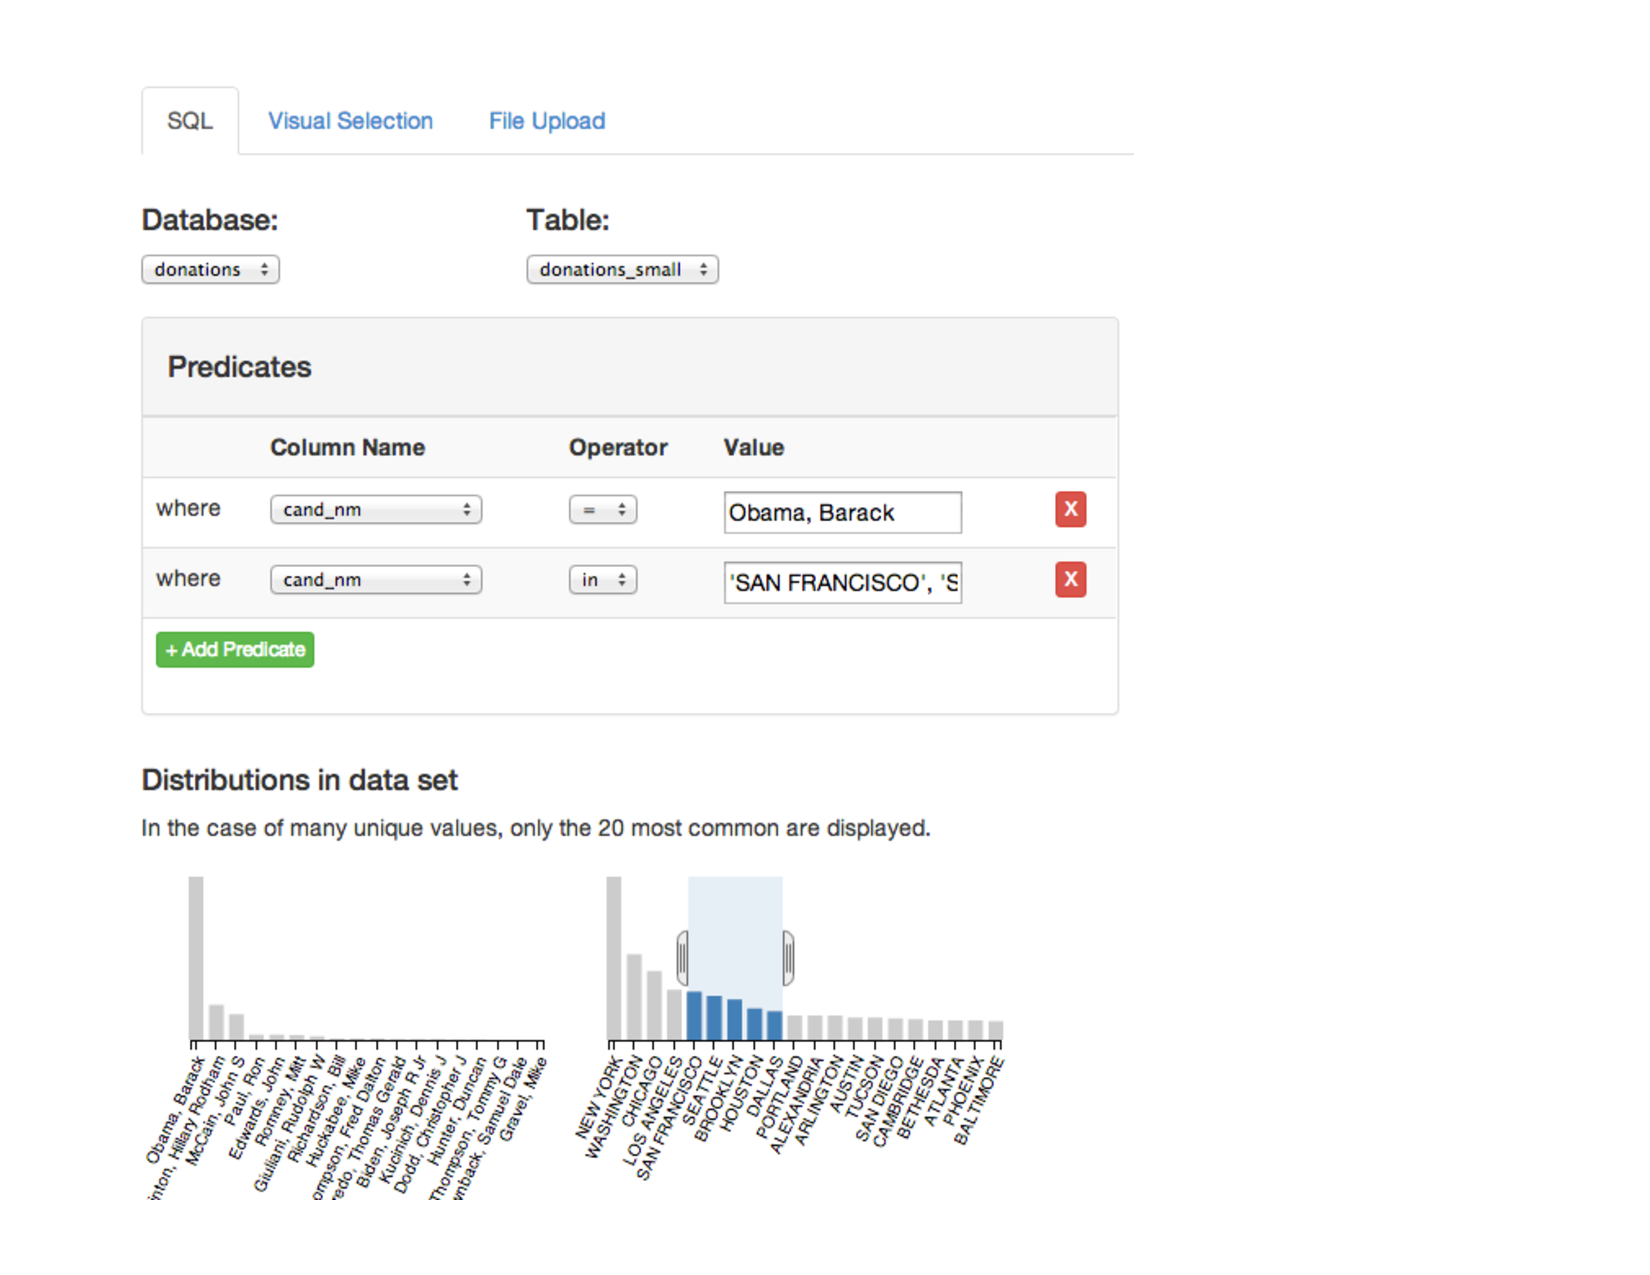
\includegraphics[trim=15mm 0mm 120mm 0mm,
clip=true]{Images/sql_builder.pdf}}}
\hbox{\resizebox{!}{6cm}{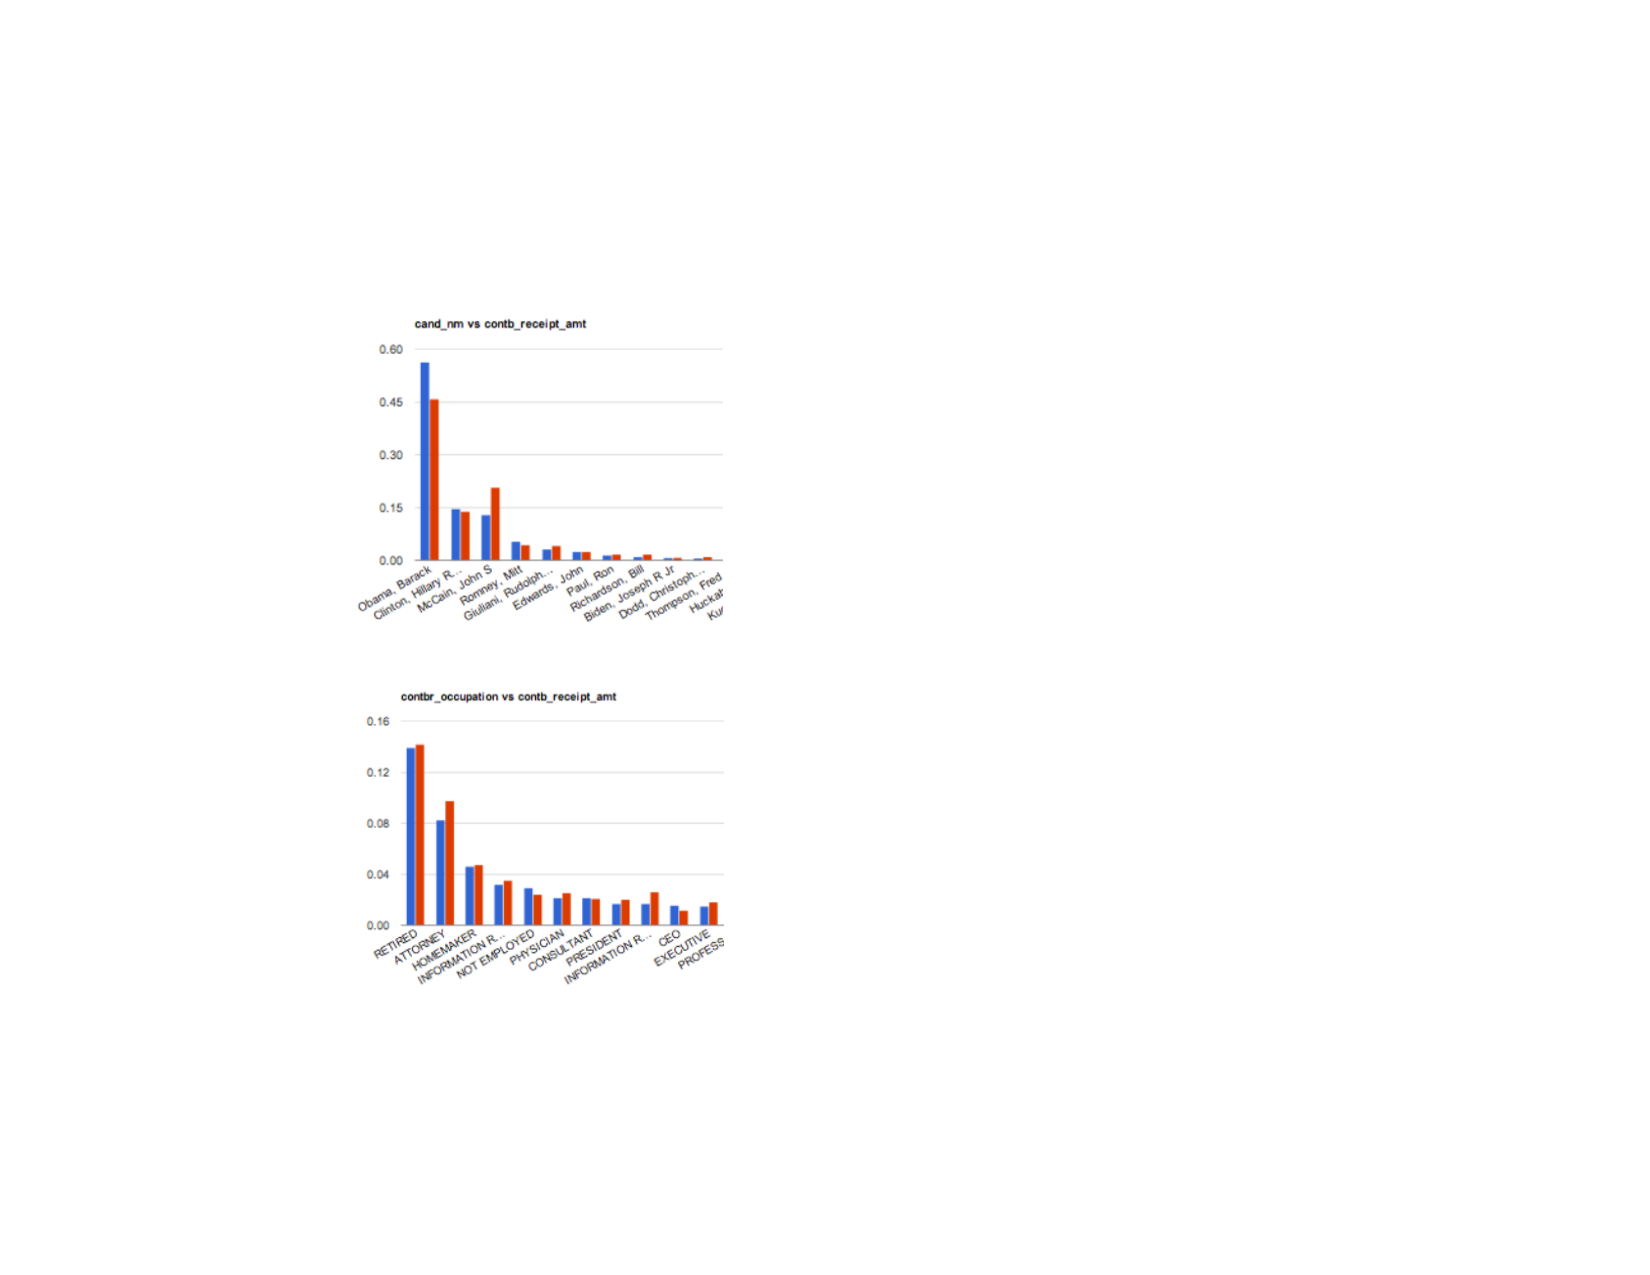
\includegraphics[trim=50mm 30mm 150mm 52mm,
clip=true]{Images/viz_panel.pdf}}}}
\caption{VizRecDB Frontend: Query Builder (left) and Example Visualizations
(right)}
\label{fig:frontend1}
\vspace{-10pt}
\end{figure} 

In this work, we focus on the \VizRecDB\ backend and develop techniques to
speed up identification of interesting views. As a result, we leave the
development of a more advanced and flexible \VizRecDB\ frontend for future work. 
In the next section, we describe the \VizRecDB\ execution engine and discuss
two implementations in detail.

%!TEX root=document.tex

\section{View Pruning}
\label{sec:pruning}

The previous sections described the \VizRecDB\ Execution Engine, the core part
of our system.
In this section, we discuss an important component of \VizRecDB\ that is invoked
even before the Execution Engine runs, namely the View Generator.
Given a user query $Q$, the purpose of the view generator module is to take the
input query, obtain metadata about the underlying tables and use correlations
between different columns in the table to prune views whose evaluation is
unnecessary. 
We distinguish between the pruning done in the execution engine and the pruning
done in the view generator: the execution engine prunes away low-utility views
while the view generator prunes away {\it redundant} views.
So what are redundant views? Redundant views are views that have similar
distributions and are therefore expected to have similar utility.
An extreme example is that of sales of a product as measured in US
Dollars and measured in Euros. Views with these measure attributes will be
identical and have the same utility.
Similarly, two dimension attributes, one corresponding to the airport name
and another corresponding to the airport code are guaranteed to produce identical
views irrespective of the measure attribute.
In both of the above cases, it suffices to compute and show only a single view
that is representative of multiple views (the frontend does list redundant
views that have been omitted).

The View Generator works in two stages: it performs view pruning offline and
identifies the set of viable views; then, when a new user query comes in, it
reads the set of viable views, performs pruning based on the input query and
passes view stubs on to the Execution Engine. 
The offline pruning does not depend on the input query and can therefore be
perfomed only once.
The offline stage works as follows. 
First, for each table, the View Generator obtains various types of
metadata including the data types of attributes, their classification into
measure and dimension attributes, number of distinct values for dimension
attributes, and the distributions for each measure attribute (mean, std
deviation).
The first piece of metadata is essential to determine the full space of
views. 
The number of distinct values for dimension attributes and the variance for
measure attributes is used to perform basic pruning of views (e.g. views
containing zero variance attributes will have low utility).
Next, the View Generator computes pairwise correlations between subsets of the
entire set of possible views.
To do so, the View Generator computes the aggregate distributions for all views
over the entire data (i.e. the comparison view). 
Once the distributions for all views have been computed, it calculates the
correlation between distributions of views that contain dimension attributes
with the same size (i.e. number of distinct values).
Specifically, since the distributions are numeric, it computes the pairwise
Pearson correlation between the distributions.
Next, it (conceptually) builds a graph of all views. 
The nodes of this graph correspond to views and an edge exists between two nodes
if the correlation between the two views is greater than a threshold (set to 0.95 in
our experiments). 
In this graph, the View Generator then identifies cliques (and almost cliques).
Observe that a clique in this graph is a set of highly correlated views,
and therefore, these views are likely to have similar utility. 
As a result, we select a
single node from each clique as a representative view for that clique and
prune the remaining views. 
We can think of this procedure as clustering views based on similarity and
choosing a representative view form each cluster.
At the end of the offline step, the View Generator stores the list of
viable views that must be evaluated at run time.

When the View Generator is invoked at runtime, it reads the list of viable
views for the table, prunes them further based on the input query (e.g.
attributes present in the where clause of the query should not be present in
any view) and passes the remaining views to the Execution Engine for
evaluation.

In real datasets, we find that the offline processing significantly
reduces the number of views that must be evaluated. 
For example, in the
diabetes dataset discussed in Section \ref{sec:experiments}, offline pruning
reduces the total number of views from XXX to XXX due to our pruning
strategy. Similarly, for the banking dataset, the total views are
reduced from XXX to XXX. In Figure \ref{}, we show graphs generated by the
View Generator for both datasets.

% \mpv{If two dimension attributes $a_i$ and $a_j$ have
% a high degree of correlation (e.g. full name of airport and abbreviated name of
% airport), the views generated by grouping the table on $a_i$ and $a_j$ will be
% very similar (and have almost equal utility). We can therefore generate and
% evaluate a single view representing both $a_i$ and $a_j$. \VizRecDB\ clusters
% attributes based on correlation and evaluates a representative view per
% cluster.}



  
% We next describe a scheme that allows us to associate upper and lower bounds for
% views by evaluating them on a small sample of the dataset.
% We describe the use of the scheme on a simple view where AVG(Y) for a given
% attribute Y is being computed for each group in attribute X.
% We can then depict this view using a bar chart or a histogram.
% 
% For this derivation, we assume that the AVG(Y) for any X = $x_i$, is normally
% distributed around a certain mean $p$.
% Given a number of samples for Y for X = $x_i$, we can employ the following
% theorem \cite{stats_book} to bound $p$ within a confidence interval with
% probability $1 - \delta$:
% \begin{theorem}~\label{thm:confint}
% If $\hat{p}$ and $s$ are the mean and standard deviation 
% of a random sample of size $n$ from a normal distribution with unknown 
% variance, a $1 - \delta$ probability confidence interval
% on $p$ is given by:
% $$\hat{p} - \frac{t_{\delta/2, n-1} s}{\sqrt{n}} \leq p \leq \hat{p} + \frac{t_{\delta/2, n-1} s}{\sqrt{n}}$$
% where $t_{\delta/2, n-1}$ is the upper 100$\alpha/2$ percentage point
% of the $t$-distribution with $n-1$ degrees of freedom.
% \end{theorem}
% 
% Now, we demonstrate how we can use this theorem to establish an upper 
% and lower bound for the utility of a view, with probability $1 - \delta$.
% 
% Let the distance vector corresponding to the target view be:
% $\bar{a} = [a_1, a_2, \ldots, a_k]$ while the distance vector corresponding to
% the comparison view is:
% $\bar{b} = [b_1, b_2, \ldots, b_k]$.
% Notice that on very large datasets, it may be beneficial to precompute the
% distance vectors corresponding to the comparison views, so we assume that the
% vector $\bar{b}$ is computed exactly and known in advance.
% We let $a = \sum_i a_i$, and $ b = \sum_i b_i$.
% 
% Our goal is to use the sample to bound the values of the $a_i$ around $\ha_i$
% such that we can establish upper and lower bounds for the utilities.
% By applying Theorem~\ref{thm:confint}, we
% can get values $c_i$ for which $a_i \in [\ha_i - c_i, \ha_i + c_i]$
% with probability greater than $1 - \delta/k$.
% (By union bound, we will be able to ensure that all $a_i$'s
% are in their intervals with probability $1 - \delta$.)
% 
% Now, given these values $c_i$, we can establish an upper bound for the
% EMD (and also similarly for other distance metrics) in the following manner:
% We let $q_1(\bar{a}) = \sum_i \ha_i - c_i$, and $q_2(\bar{a}) = \sum_i \ha_i + c_i$.
% 
% 
% \begin{align*}
% EMD(\bar{a}, \bar{b}) & = \sum_i |a_i / a - b_i / b|\\
%           & = \sum_i |a_i / a - b_i / b|\\
%           & = 1/ab \sum_i \max (a_ib  - b_ia, b_ia - a_ib)\\
% \end{align*}
% Thus, we have:
% \begin{align}
% \frac{1}{b q_1(\bar{a})} \sum_i \max (a_ib  - b_ia, b_ia - a_ib) \leq & EMD(\bar{a}, \bar{b}) \leq \frac{1}{b q_2(\bar{a})} \sum_i \max (a_ib  - b_ia, b_ia - a_ib)\label{eq:emd}
% \end{align}
% 
% Note that: 
% \begin{align*}
% (\ha_i - c_i)b  - b_i (\sum_i (\ha_i + c_i)) & \leq a_ib  - b_ia  \leq (\ha_i + c_i)b  - b_i (\sum_i (\ha_i - c_i)), \textrm{\ and} \\
% b_i (\sum_i (\ha_i - c_i)) - (\ha_i + c_i) b & \leq b_i a  - a_i b  \leq  b_i (\sum_i (\ha_i + c_i)) - (\ha_i - c_i) b
% \end{align*}
% By plugging these quantities back into Eq~\ref{eq:emd},
% we have upper and lower bounds on the EMD metric.
% Similar mechanisms may be used to derive upper and lower bounds for other metrics.
% 
% Now that we have upper and lower bounds for the utility of each target view
% by evaluating the query on a sample,
% we can easily use it to prune away a number of views that are definitely not likely to be part 
% of the top-K,
% and instead focus on views that may be part of the top-K.

%   \subsection {Partitioning Tables}
%   The increase in the total execution time when a large number of queries are
%   executed in parallel suggests that there is a ``sweet spot'' with respect to
%   the maximum number of queries that can be run in parallel on a given table.
%   Therefore, we uniformly partition large tables into smaller ones and run
%   subsets of queries against each of the partitions. Note that the views
%   returned are nor approximate because we are now executing views against
%   subsets of the data. As a result, bounds developed in sampling now apply. We

 


%If a dimension attribute $\mathcal{d}$ is highly correlated with measure
  %attribute $\mathcal{m}$, then?

% \mpv{also from full paper draft}
% It is possible to collect the above statistics at the dataset level too, as
% opposed to the entire table level. The advantage of table level statistics is
% that they have to be computed only once per table; however, dataset-level
% statistics are more accurate since they only consider the specific parts of the
% table. XXX: we use dataset-level statistics with table statistics do not result
% in aggressive pruning. 




%  
% 
\section{Handling attributes of different kinds}
\mpv{Numerical, Temporal, Categorical, Gepgraphical}\\
\mpv{Binning}
%\section{Handling distribution of single attributes}
%!TEX root=document.tex

\section{User Study}

We demonstrate the utility of \SeeDB\ through a user study on MTurk as well as
through in person interviews with data analysis experts. 
Our goals with the user study were as follows: (1) to validate the \SeeDB\
technique of identifying interesting views via deviation; (2) to evaluate the
relative merit of different distance metrics; and (3) to evaluate the \SeeDB\
tool as a whole.

To study questions (1) and (2), we created an MTurk study where 30 turkers were
provided with a questionnaire containing 20 visualizations. These visualizations
had differing utilities and varying number of distinct values on the X axis
(see Figure \ref{}) for examples of visualizations. For each visualization, we
asked subjects to rate (on a scale of 1 to 5) if the visualization showed
something interesting or insightful about the underlying data. We removed the X
and Y axis labels to avoid confusing the subjects. The results are shown in
Table \ref{}. We see that XXX. 

We also used the data from this study to evaluate the
merit of different kinds of utility metrics. Specifically, we ranked the set of
visualizations shown to the subjects using different metrics (see Section
\ref{}).
We then compared the ranking of visualizations generated by the metrics to the
rating provided by the users. 
To convert the rankings to ratings, we divided the ranked list of visualizations
into 5 bins. The top ranked bin corresponded to a rating of 5 while the lowest
ranked bin corresponded to a rating of 1.
We see that XXX.

To study the utility of \SeeDB\ as a whole, we conducted in-person interviews
with XXX experts in data analysis. We adopted the following protocol: 

% \stitle {Scenario 1: Demonstrating Utility.} Attendees are provided with three
% diverse, real-world datasets to explore using \SeeDB. For each dataset,
% attendees can issue ad-hoc or pre-formulated queries to \SeeDB. \SeeDB\ will
% then intelligently explore the view space and optimize query execution to return the
% most interesting visualizations with low latency. Attendees can examine the
% returned queries visually, via the associated view metadata, and via
% drill-downs. To aid the evaluation of visualizations, the demo system will 
% be configured to also show the user ``bad'' views (views with low utility) that were not selected
% by \SeeDB.
% Similarly, we provide pre-selected queries (and
% previously known information about their results) to allow attendees to
% confirm that \SeeDB\ does indeed reproduce known information about these
% queries. Attendees will also be able to experiment with a
% variety of distance metrics for computing utility and observe the effects on the
% resulting views.

% \stitle{Scenario 2: Demonstrating Performance and Optimizations.} This scenario
% will use an enhanced user interface and synthetic datasets mentioned above.
% Attendees will be able to easily experiment with a range of synthetic datasets and input
% queries by adjusting various ``knobs'' such as data size, number of attributes, and
% data distribution. In addition, attendees will also be able to select the
% optimizations that \SeeDB\ applies and observe the effect on response times and
% accuracy.

% Thus, through our demonstration of \SeeDB\, we seek to illustrate that (a) it is
% possible to automate labor-intensive parts of data analysis, (b) aggregate
% and grouping-based views are a powerful means to identify interesting trends
% in data, and (c) the right set of optimizations can enable real-time data
% analysis of large datasets.
%!TEX root=document.tex

\section{Experimental Evaluation}

We evaluated the performance of \VizRecDB\ on a variety of real and synthetic
datasets as shown below. 
In particular, we evaluated the performance of our
DBMS-backed execution engine as well as our in-memory execution engine, and the
respective optimizations. 
For the DBMS-backed engine, we also built an analytical model to help pick
parameters for \VizRecDB.

\subsection{Experimental Setup}

\begin{table}[htb]
  \centering \scriptsize
  \begin{tabular}{|c|c|c|c|c|c|c|} \hline
  Type & Dataset & Num  & Num  & Num  & Size (GB) &
  Num \\
  & Name & Rows & Dimensions &  Measures & & Views \\ \hline 
   & $Small_1$ & 1M & 5 & 2 &  0.1 & \\ 
  Small & $Small_2$ & 10M & 5 & 2 &  1 & 10\\ 
   & $Small_3$ & 100M & 5 & 2 &  10 & \\ \hline
   & $Med_1$ & 1M & 50 & 5 &  0.4 & \\
  Medium & $Med_2$ & 10M & 50 & 5 &  4 & 250\\ 
   & $Med_3$ & 100M & 50 & 5 &  40 & \\ \hline
   & $Large_1$ & 1M & 100 & 10 &  1 & \\
  Large & $Large_2$ & 10M & 100 & 10 &  10 & 1000\\
   & $Large_3$ & 100M & 100 & 10 &  100 & \\ \hline
  \end{tabular}
  \caption{Datasets used for testing}
  \label{tab:datasets} 
\end{table}

Table \ref{tab:datasets} lists the datasets on which we evaluated the
performance of \VizRecDB. These datasets are synthetically generated and their size
varies from 100 MB to 100 GB and number of attributes ranges from 5 - 100 dimension attributes and 2 -
 10 measure attributes. The relative cardinality of dimension and measure attributes
was chosen to model real-world datasets which usually have a large number of
dimension attributes but few measure attributes. To accurately estimate the
effect of specific optimizations, for each dataset, we also created a
supplemental dataset with the same specifications except that each attribute had
the same number of distinct values (100).

For each dataset, we used \VizRecDB\ to find the top 20 views of the input query.
Any run that took more than 1 hour was terminated. All experiments were repeated
three times and the results were averaged.
We ran experiments using Postgres as the backend database for \VizRecDB\ and a single
machine with 32 Intel Xeon E7 processors with hyperthreading enabled and 256 GB
RAM.

\subsection{DBMS-backed Execution Engine}

We now present experimental characterization of the optimization
strategies described for the DBMS-backed execution engine (
\ref{subsec:VizRecDB_backend}).
Our goal is to understand the effect of each strategy on \VizRecDB\ performance. We
also build an analytical model and predict the optimal set of
parameters for \VizRecDB.

\subsubsection{Basic Framework}
We first examined the baseline performance of \VizRecDB\ without any optimizations.
For each possible view, we executed the target and comparison view queries
separately and sequentially, and then picked the top views. This corresponds to
the basic framework described in Section \ref{sec:basic_framework}. The number
of queries executed for each dataset was twice the number of views shown in
Table \ref{tab:datasets}. Figure \ref{fig:baseline_performance} shows the baseline
performance for Small, Medium and Large datasets of size 1M. We observe that
execution time increases super-linearly as the size of the dataset (number of dimension and
measure attributes) increases. Moreover, as mentioned before, even for the
Medium sized dataset (1M rows, 5 measure and 50 dimension attributes), \VizRecDB\
execution takes 700s, a latency that is unacceptable for interactive queries.

\begin{figure}[h]
  \centering
    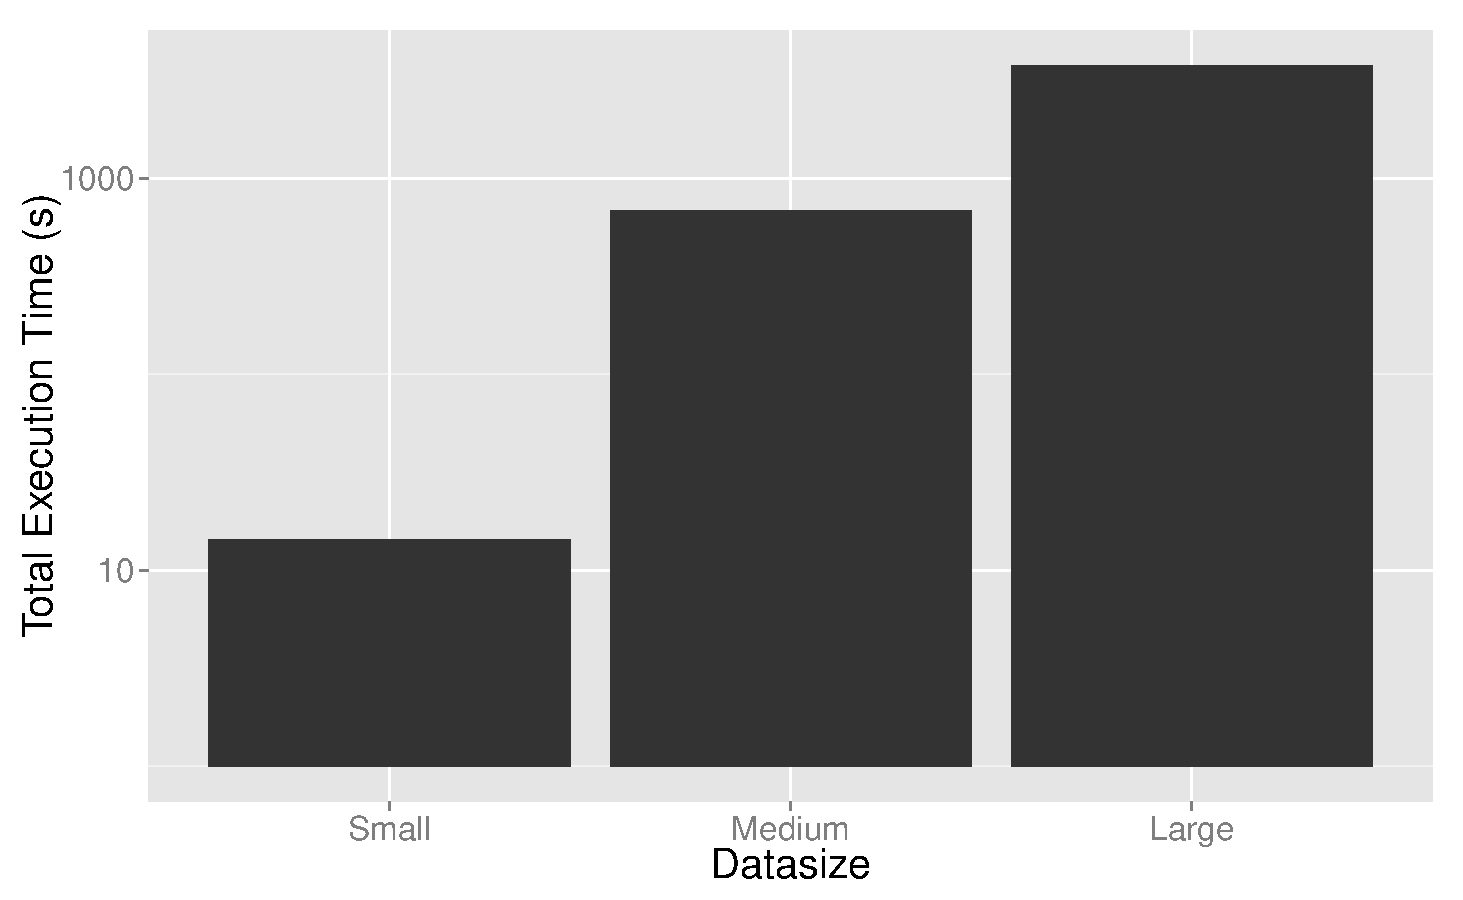
\includegraphics[width=6cm]{Images/baseline_performance.pdf}
    \caption{Baseline Performance} 
      \label{fig:baseline_performance}
\end{figure}

\subsubsection{Combine target and comparison view query}
Next, we study the effect of combining target and comparison view queries as
described in Section \ref{subsec:target_comparison_view}. The goal of this
optimization is to execute both queries in a single scan of the table.
Therefore, the total number of queries executed is equal to the number of
views possible for a given dataset. This optimization offers an average speed up
of 1.7x across a range of selectivities for the input query.

\subsubsection{Combine Multiple Aggregates}
\VizRecDB\ uses the parameter $n_{agg}$ to denote the number of aggregates that may
be included in the same view query. Therefore, given a set of view queries with
the same group-by attribute, view queries are combined so that each query has up
to $n_{agg}$ aggregates. We varied $n_{agg} \in {2, 3, 5, 10}$ for each dataset
(Note that the Small and Medium dataset have only 2 and 5 measure attributes
respectively).
Figure \ref{fig:mult_agg} shows the performance gains achieved for the 1M row
datasets. We see that for a given dataset, increasing $n_{agg}$, i.e. computing
more aggregates in the same query, gives an almost linear speedup. We also
notice that this optimization is slightly more effective for larger datasets.

\begin{figure}[h]

  \centering
    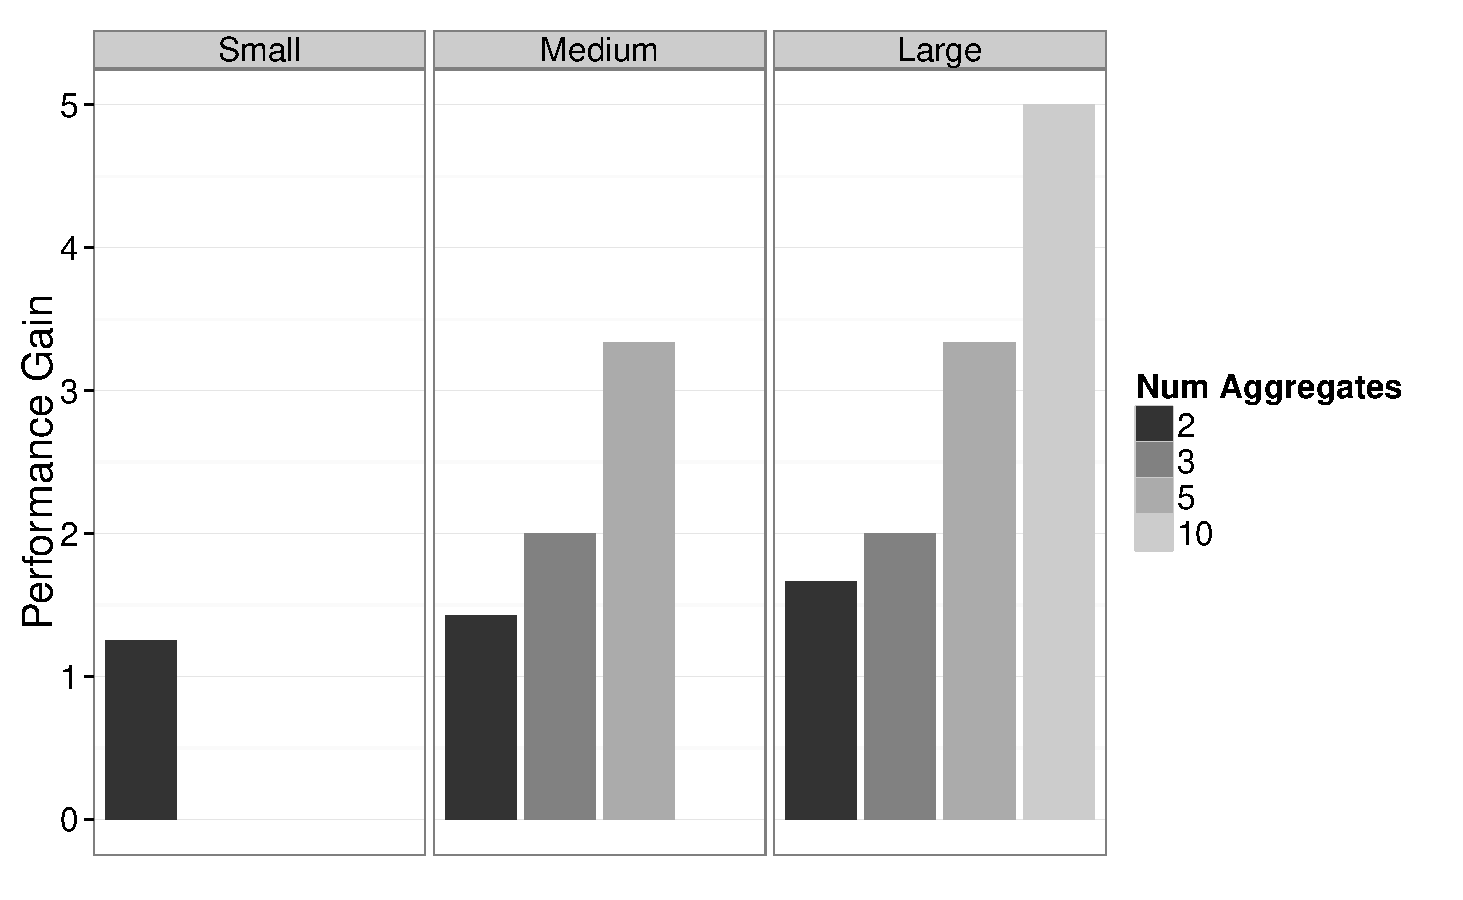
\includegraphics[width=6cm]{Images/mult_agg.pdf}
    \caption{Effect of Multiple Aggregate Optimization} 
      \label{fig:mult_agg}
\end{figure}

\subsubsection {Parallel Query Execution}
As discussed in Section \ref{subsec:parallel_exec}, executing view queries in
parallel can provide significant performance gains; however, a high degree of
parallelism can lead to a performance drop off for several reasons. Potential
reasons include disk contention, RAM usage, lock contention, context switches
and cache line contention
\cite{Postgres_wiki}.
Identifying the right amount of parallelism requires tuning for the particular
workload. The \VizRecDB\ workload consists of multiple parallel queries performing
full sequential scans of a given table. To evaluate the
effect of parallelism, we varied the number of queries that can be executed in
parallel and measured its effect on the average time to execute a query as well
as the total execution time. Since our backend DBMS is Postgres, parallel query
execution is implemented by opening multiple connections and running queries
sequentially on each connection.

Figure \ref{fig:parallelism} shows the effect of parallelism on the average
execution time per view (Medium dataset, 1M rows). Note the log scale on the
y-axis.
We observe that query execution time stays flat between 1 - 10 connections, suddenly increases between
10 - 20 connections, and then increases linearly for more than 20 connections.
This suggests that the benefits of parallel execution are outweighed by
contention beyond 20 connections. Figure \ref{fig:parallelism_total} shows the
total time (as opposed to per view execution time) taken by \VizRecDB\ for varying
levels of parallelism. We observe that the minima occurs in the range between 10
- 20 parallel queries and the execution times flatten out after 40 parallel
queries.
This trend is the effect of two opposing factors: (A) increased parallelism
increases contention, and therefore increases per query execution time, and (B)
parallelism decreases the number of batches of queries that must be executed,
thus reducing overall time.
We will take these two opposing forces into account when we develop an
analytical model for \VizRecDB\ execution time in Section \ref{sec:model}.

\begin{figure}[h]
  \centering 
    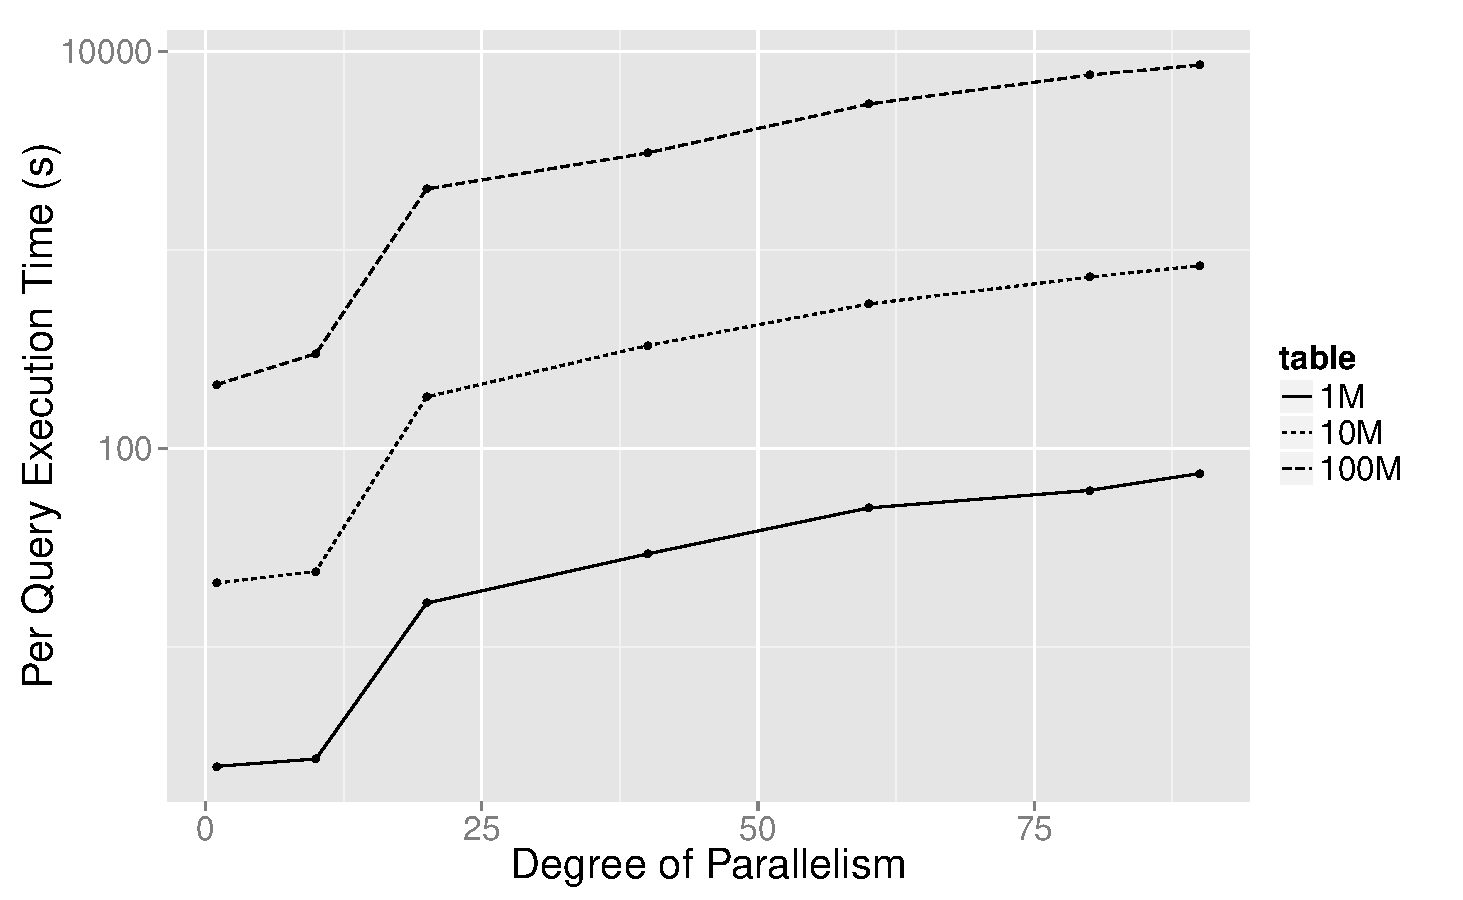
\includegraphics[width=6cm]{Images/parallelism.pdf}
      \caption{Effect of Parallelism on Per View Execution Time} 
        \label{fig:parallelism}
\end{figure}



\begin{figure}[h]
  \centering
    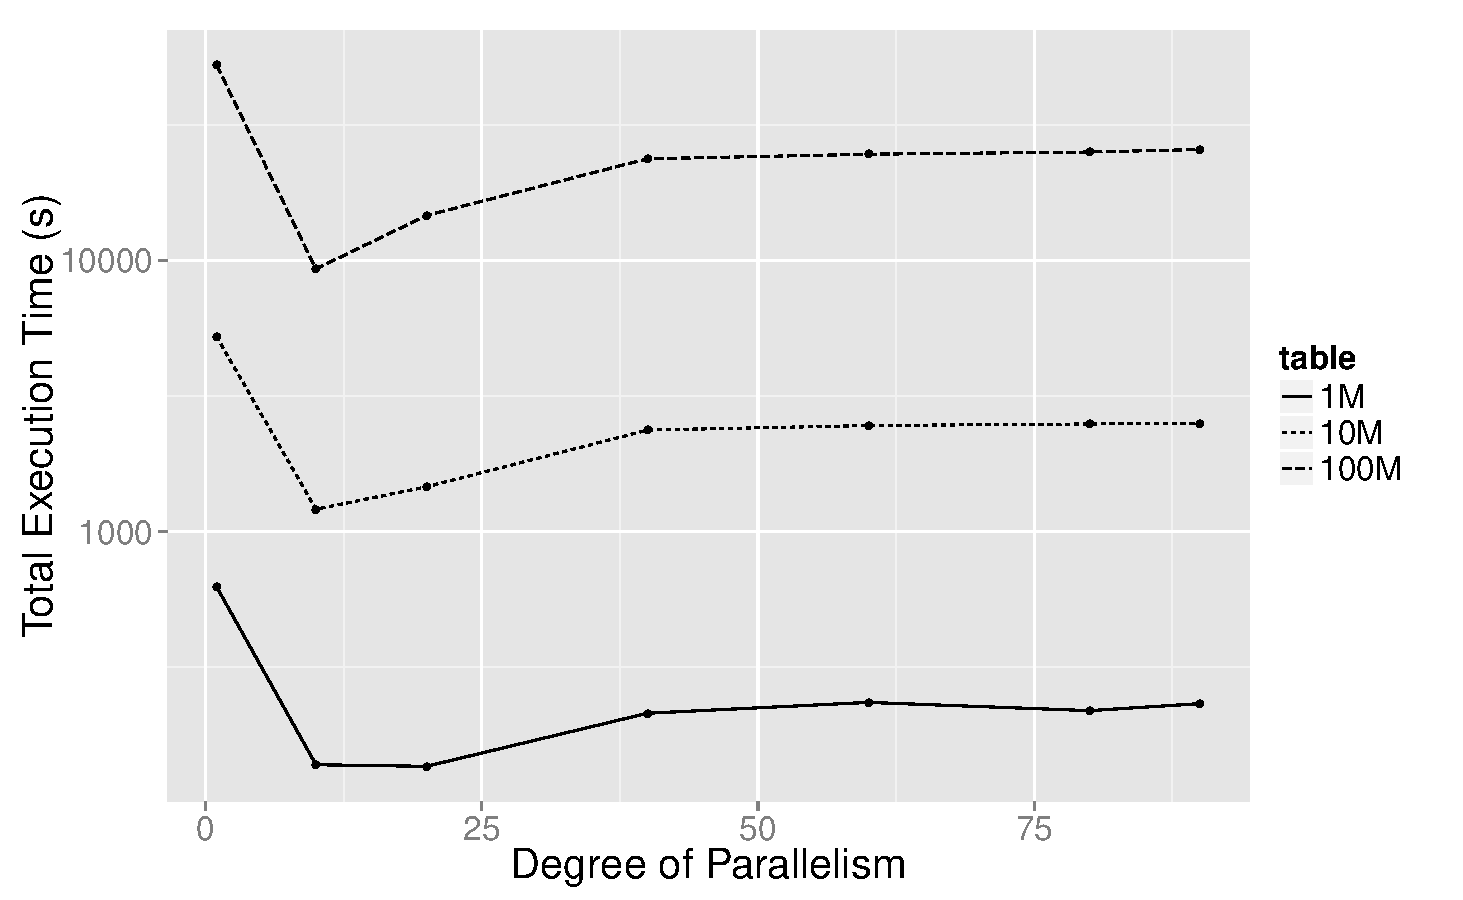
\includegraphics[width=6cm]{Images/parallelism2.pdf}
  \caption{Effect of Parallelism on Total Execution Time} 
    \label{fig:parallelism_total}
\end{figure}

\subsubsection {Combine Multiple Group-bys}
\label{subsec:mult_gb_expt}
Combining multiple attributes in a group-by clause can reduce the number of
views that must be explored individually.
However, the benefits of this optimization can be lost to high intermediate
result cost if the number of distinct groups is large. As mentioned before, we
divide this optimization into two phases:
(1) {\it Temp Table Creation} and (2) {\it Temp Table Querying}. In the first
phase, we run queries with grouping based on multiple attributes and store the
results in temporary tables. In the second phase, we run single
aggregate+group-by queries on the temp tables to obtain final results for views.
For instance, suppose that we want to compute the results for views ($a_1$, $m$,
$f$), ($a_2$, $m$, $f$) and ($a_3$, $m$, $f$). Instead of executing these views
individually, we combine these three views into a single view, (\{$a_1$, $a_2$,
$a_3$\}, $m$, $f$), which computes the aggregate for attribute $m$ using
function $f$ and groups by the attributes \{$a_1$, $a_2$, $a_3$\}. The results
of this query are stored in a temporary table which is then queried to get
results for the original views, ($a_1$, $m$, $f$), ($a_2$, $m$, $f$) and ($a_3$,
$m$, $f$).

\VizRecDB\ uses the parameter $n_{GB}$ to denote the number of attributes in the
group-by clause. To evaluate the effect of combining group-bys, we ran \VizRecDB\
by varying number of group-by attributes, i.e. the $n_{GB}$ parameter, between 1
and the number of dimensions $d$ in a given table. For each run, we measured the
amount of time taken to create the temporary tables, the time taken to query the
temporary tables and the total execution time. Figure
\ref{fig:avg_tt_creation} to \ref{fig:total_time} show the
results for the Medium dataset of size 1M tuples.

{\bf Temp Table Creation Phase}: Figure \ref{fig:avg_tt_creation} shows the
average time required to create temporary tables for $n_{GB}$=1\ldots50. There
are several points to note in this graph: (1) for $n_{GB}>=10$, the number of
connections does not have a significant impact of the temp table creation time.
We see this behavior because for $n_{GB}>=10$, the number of temp tables created
is $<=5$ and therefore a maximum of 5 connections is used irrespective of the
number of connections that are open.
We also note an upward trend in the total temp table creation time with
increasing $n_{GB}$ because the temporary tables gradually become larger in size
(the number of rows in the table is bounded by the number of rows in the input
table but an increase in $n_{GB}$ increases the columns present in the table).
We also observe that the ``sweet spot'' for temp table creation occurs between 1 -
2 group-bys. 

% Note that the time required for temp table creation is roughly
% proportional to the size of the temp tables. We leverage this fact when we
% develop the analytical model in the next section.

\begin{figure}[h]
  \centering
    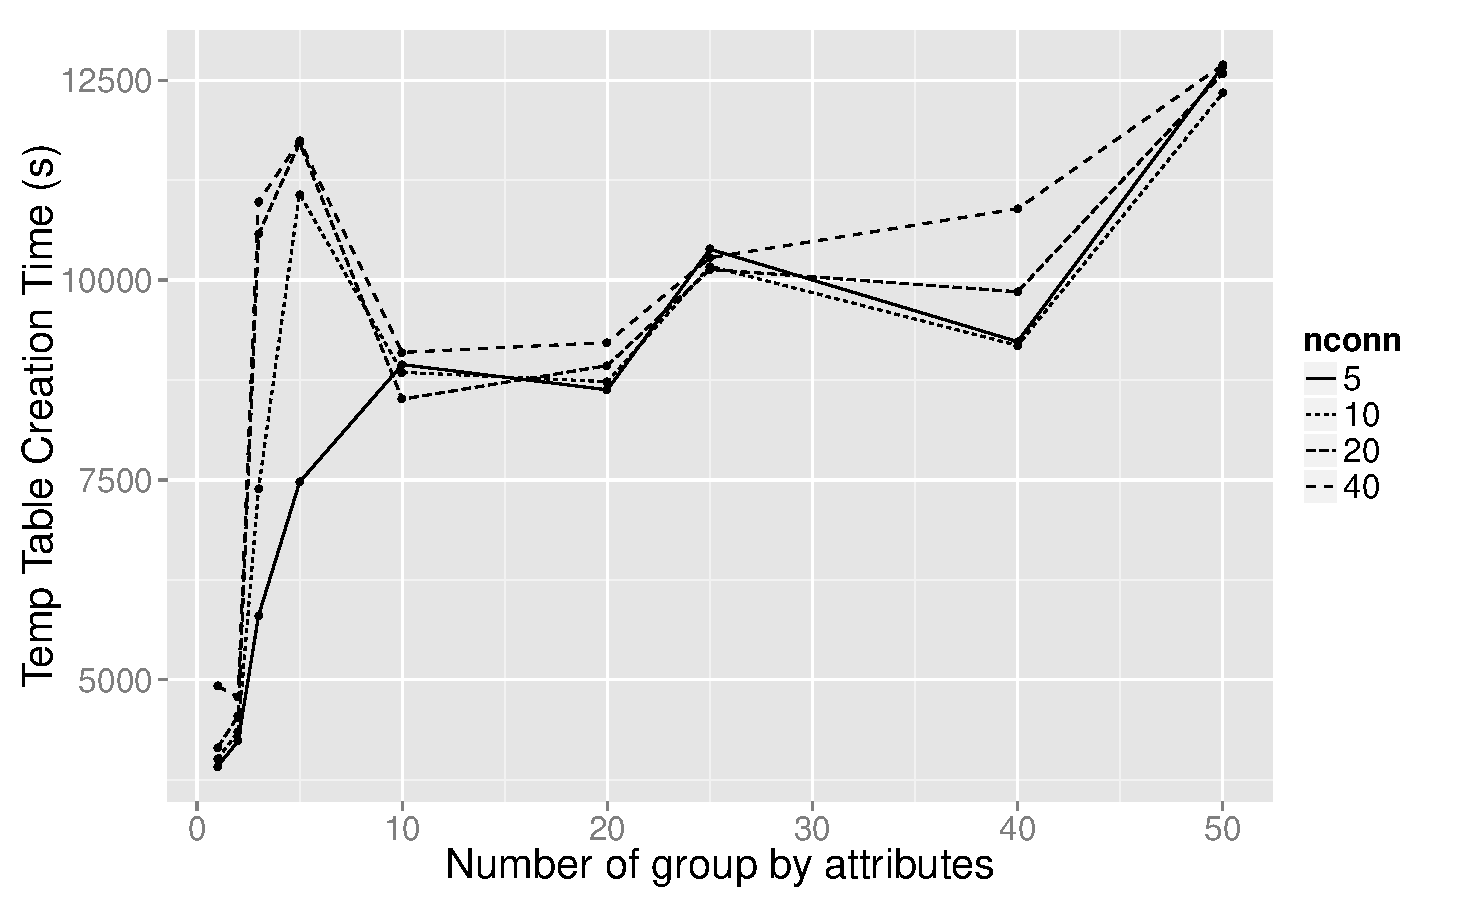
\includegraphics[width=6cm]{Images/mult_gb_tt_creation_single.pdf} 
  \caption{Average Temp Table Creation Time} 
    \label{fig:avg_tt_creation}
\end{figure}

\begin{figure}[h]
  \centering
    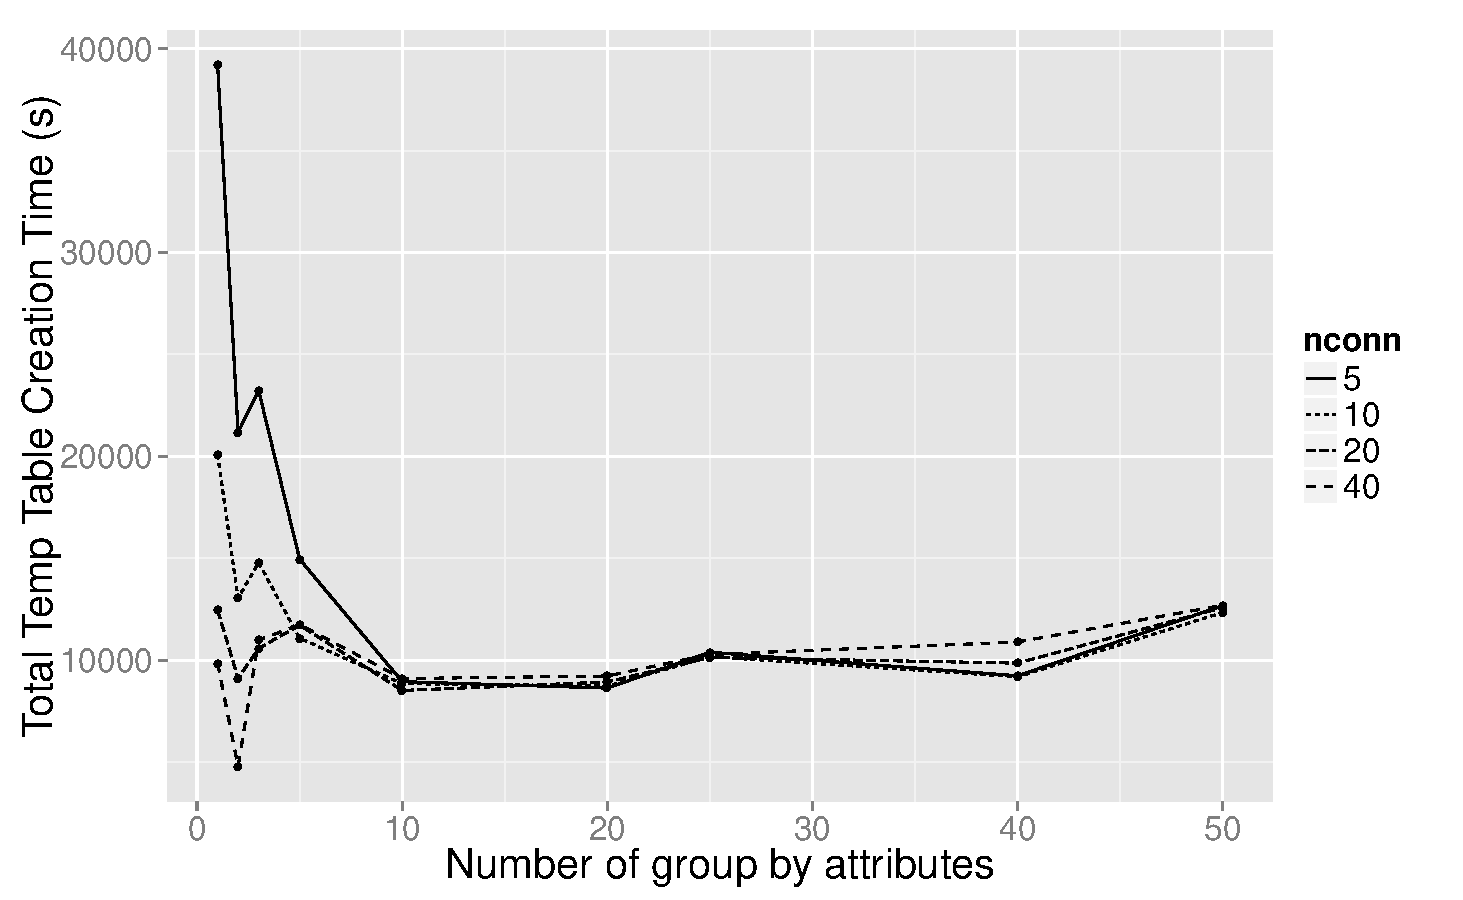
\includegraphics[width=6cm]{Images/mult_gb_tt_creation_total.pdf}
  \caption{Total Temp Table Creation Time} 
    \label{fig:total_tt_creation_time}
\end{figure}

Figure \ref{fig:total_tt_creation_time} shows the total time spent in creating
temporary tables in \VizRecDB. As before, we see that the total time
flattens out after 10 group-bys; however, we observe a reordering of the the
trend lines with respect to number of connections. While the average time taken
to generate temp tables with 5 connections is the least, \VizRecDB\ must run more
batches of queries to create the required number of temporary tables. We observe
that that 40 connections is optimal for minimizing the total temp table creation
time. As in the previous diagram, we observe a minima around $n_{GB}=2$.

{\bf Temp Table Query Phase}: Figures \ref{fig:avg_tt_query_time} and
\ref{fig:total_tt_query_time} respectively show the average time required to run
each view query on the temp tables and the total time to run all view queries.
Note that for the Medium dataset, there are 250 possible views and therefore 500
view queries that are to be run against the database.

In Figure \ref{fig:avg_tt_query_time}, we see clear trends in  the average time
taken to execute view queries on temp tables. Specifically: (1) The time taken
to query a temp table increases non-linearly with the number of queries
executing in parallel. We see that the trend lines are ordered by number of
connections and the loss of performance grows with number of connections. (2) As
before, we observe a slight increase in the execution time as the size of temp
tables increases. This is not surprising since the query executor must scan and
process more data. (3) Finally, we observe a minima at $n_{GB}=2$, similar the to
two graphs above.


\begin{figure}[h]
  \centering
    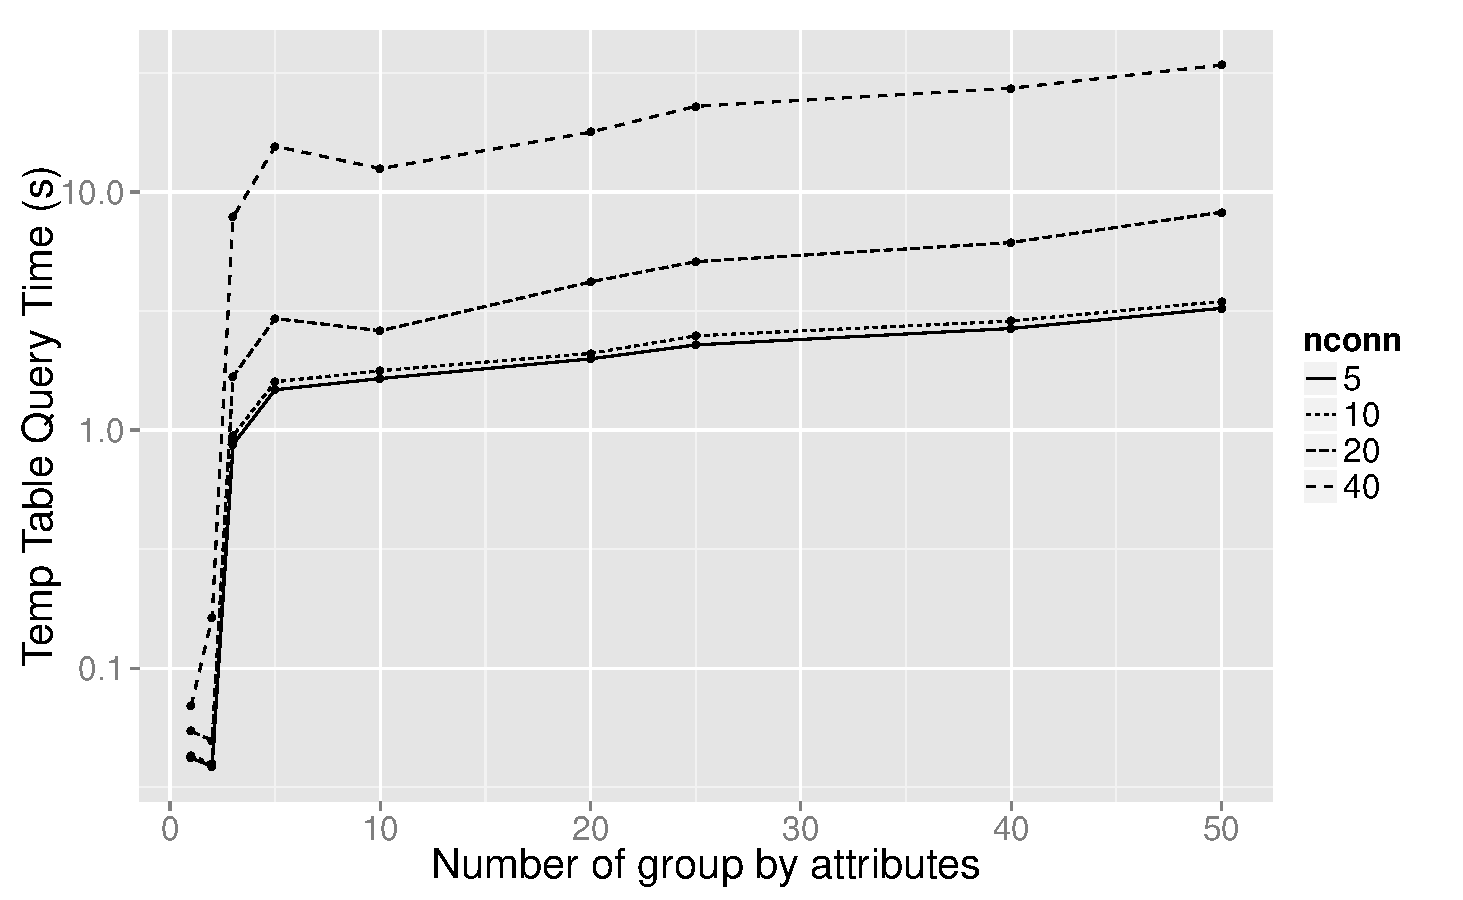
\includegraphics[width=6cm]{Images/mult_gb_tt_query_single.pdf}
  \caption{Average Temp Table Query Time}
  \label{fig:avg_tt_query_time}
\end{figure}

\begin{figure}[h]
  \centering
    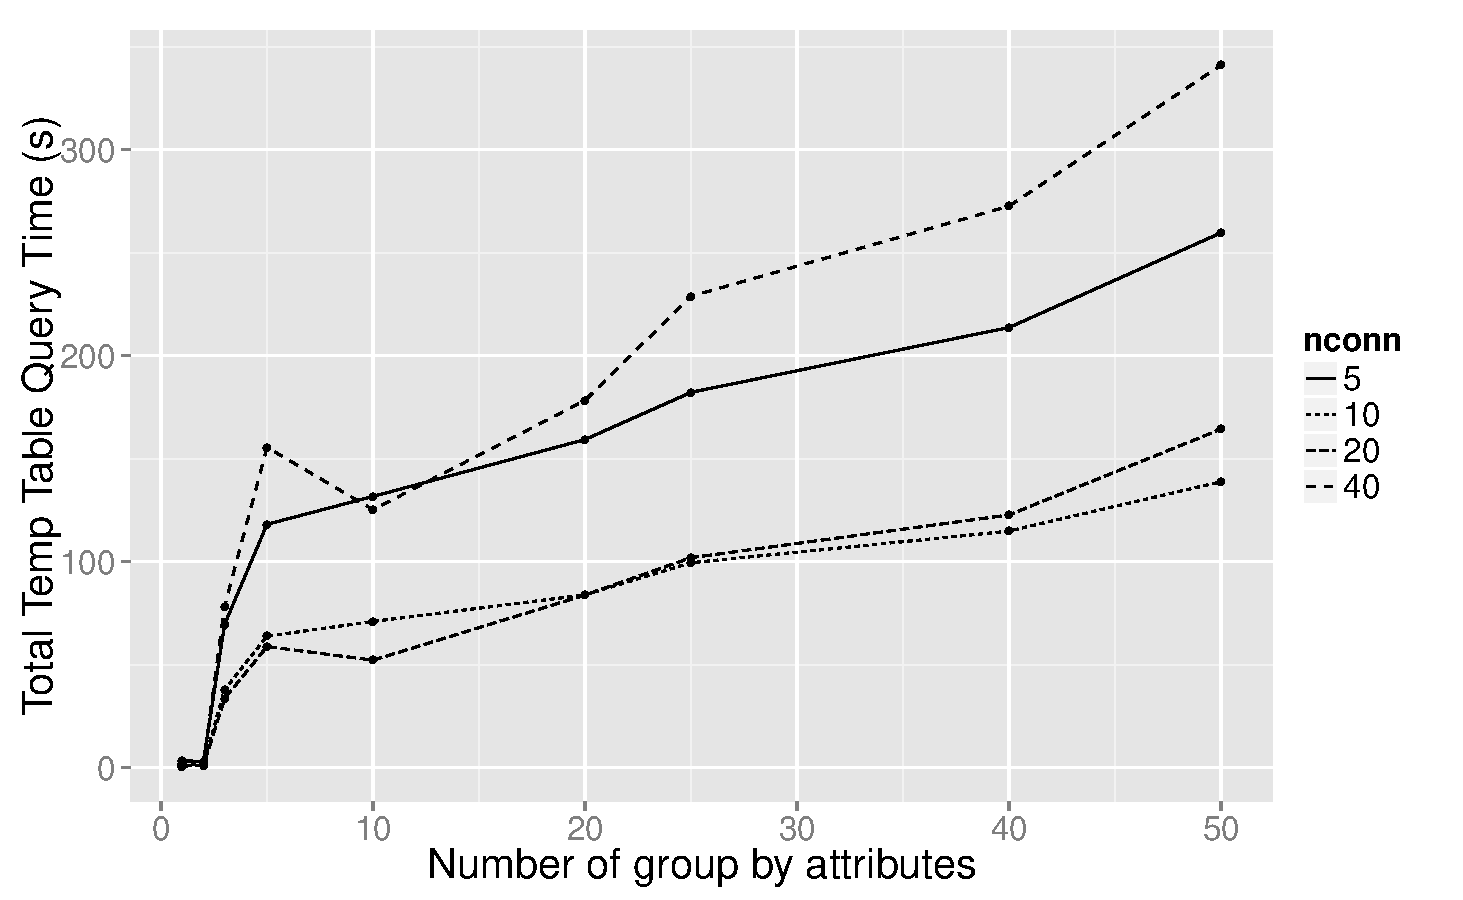
\includegraphics[width=6cm]{Images/mult_gb_tt_query_total.pdf}
     \caption{Total Temp Table Query Time} 
       \label{fig:total_tt_query_time}
\end{figure}

Figure \ref{fig:total_tt_query_time} shows the total time taken to query the
temp tables for all the final views. Note again that the trends in total query
time are not identical to those in average query time because number of query
batches required is inversely proportional to the number of connections.
In Figure \ref{fig:total_tt_query_time}, we see that runs with 5 connections are
slow not because of high average query time but because of the large number of
batches of queries that must be executed. In contrast, runs with 40 connections
require very few batches but have high average query time. 10 - 20 connections
and $n_{GB}=1-2$ achieves the best performance.



{\bf Total Execution Time}: The total execution time for \VizRecDB\ is the sum of
time required for the two phases above. Figure \ref{fig:total_time} shows the
total \VizRecDB\ execution time for different values of $n_{GB}$ and number of
connections. We observe that the best performance is obtained for
$n_{GB}=2$ and 40 parallel connections.

\begin{figure}[h]
     \centering
    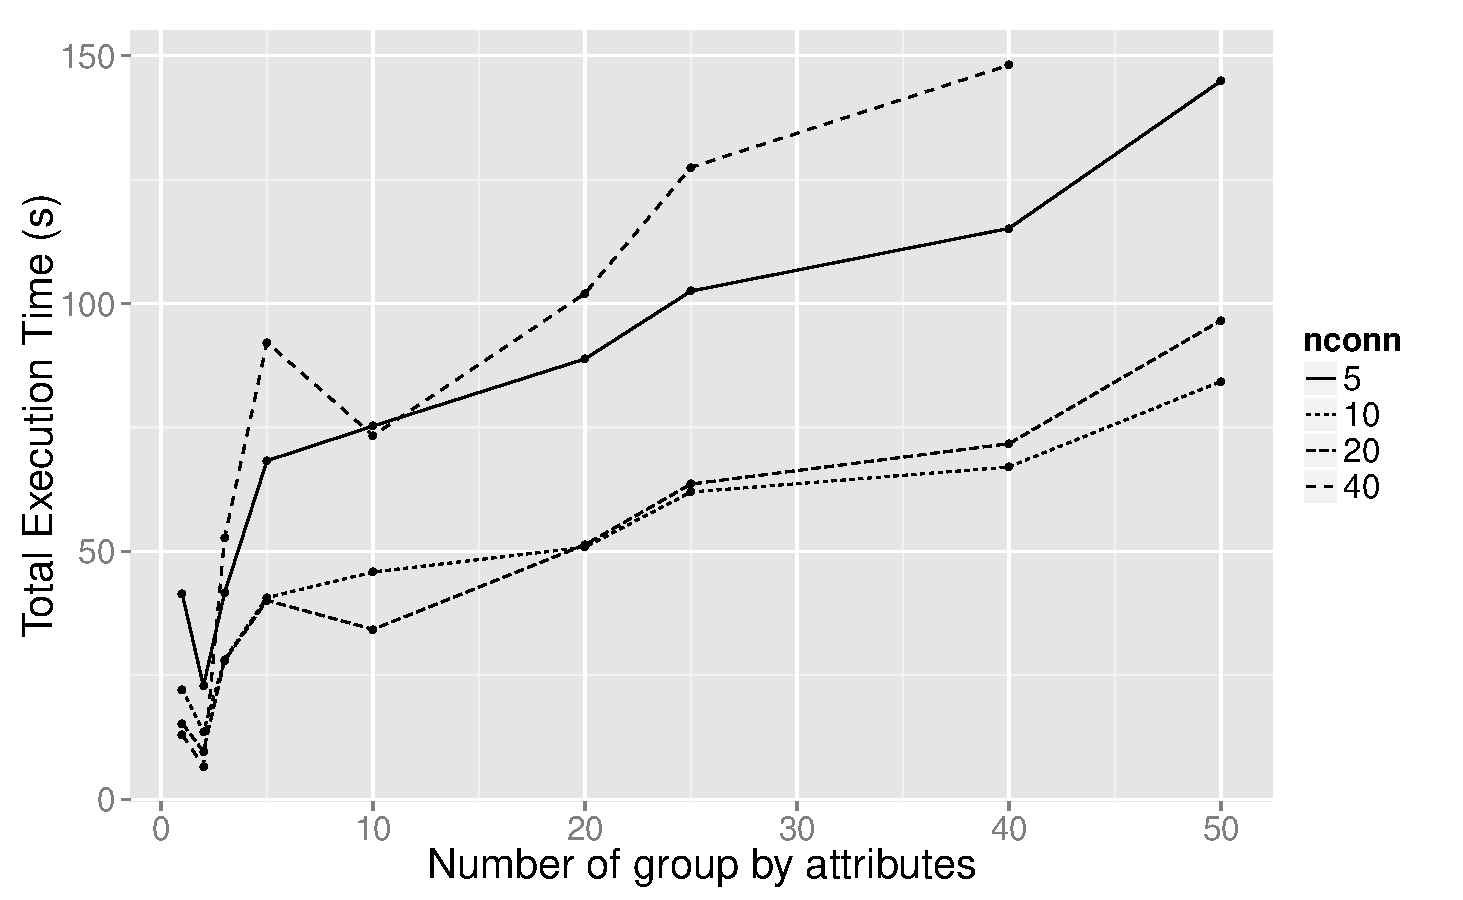
\includegraphics[width=6cm]{Images/mult_gb_total.pdf}
    \caption{Total Execution Time}
  \label{fig:total_time}
\end{figure}

\begin{figure}[h]
  \centering
    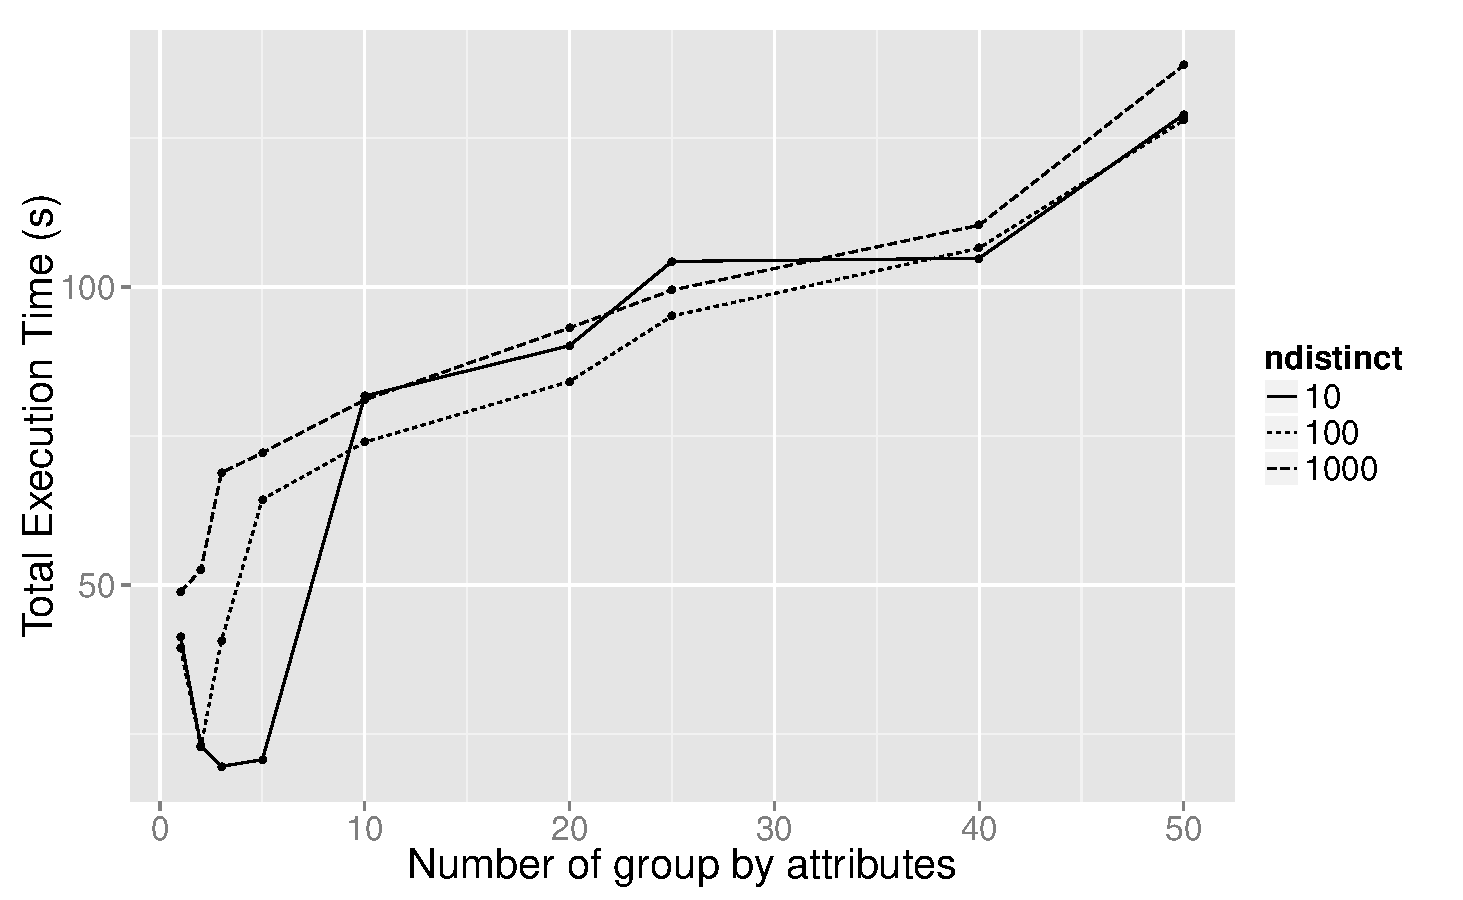
\includegraphics[width=6cm]{Images/mult_gb_diff_distinct.pdf}
    \caption{Total Execution Time vs. Number of Distinct Values} 
  \label{fig:total_time_diff_distinct}

\end{figure}

{\bf Effect of Number of Groups:} The above experiments suggest that $n_{GB}=2$
is the optimal value for the number of group by attributes, both for temp table
creation and querying.
Next we study whether this constraint applies to the number of attributes in the
group by clause or the number of distinct groups produced by the grouping. For
this purpose, we created variants of the Medium dataset (1M rows) where each
dimension attribute had $n$ distinct values with $n$=10\ldots1000. We then
repeated the experiments combining multiple group-bys using these datasets.
Figure \ref{fig:total_time_diff_distinct} shows the results of this test. In the
test dataset, the total number of distinct groups for attributes $a_i$ and $a_j$
is the product of the number of distinct groups for each attribute. We observe
in \ref{fig:total_time_diff_distinct} that the previously-observed minima at
$n_{GB}=2$ is actually a function of the number of distinct groups that are
generated by the multiple-attribute grouping.
Specifically, we observe that the optimal value for the number of distinct
groups is in the range of 10,000 - 100,000. We observe similar trends for temp
table creation and query time.



\subsubsection{Analytical Model}
\label{sec:model}
In this section, we use insights from the experimental characterization of
various optimizations to develop an analytical model of \VizRecDB\ performance.
Table \ref{tab:model_params} defines the various parameters used in our model.

\begin{table}
{\center
\vspace{-10pt}
\begin{tabular}[h]{|c|p{5.5cm}|}
\hline
Parameter & Description \\ \hline
$d$ & Number of dimension attributes in table \\
$n$ & Number of rows in input table \\
$n_{tt}$ & Number of rows in temporary table \\
$c_{tt}$ & Number of columns in the temporary table \\
$t_r$ & Time to access a single row of any table \\
$t_c$ & Time to process a single column in a row \\
$t_w$ & Time to write a single row of a table \\
$n_{agg}$ & Number of aggregate attributes computed in a single query \\
$n_{d_{i}}$ & Number of distinct values in attribute $d_i$ \\
$T_{create}$ & Time required to create a temp table \\
$T_{query}$ & Time required to query a temp table \\ 
$b_{create}$ & Number of batches of queries required to create temp tables \\
$b_{query}$ & Number of batches of queries required to query temp tables \\
$n_{conns}$ & Number of queries executing in parallel \\ \hline
\end{tabular}
\vspace{-10pt}
\caption{Analytical model parameters \label{tab:model_params}}
}
\end{table}

% As before, consider the two stages of processing: {\it Temp Table Creation} and
% {\it Temp Table Querying}. In \VizRecDB\, these two stages take place in parallel:
% first, we create a set of temp tables; then we query the temp tables and as we
% finish querying existing tables, we create new tables. The creation of new
% tables and querying of old tables happens in parallel. 

As before, we break our model into two parts, {\it Temp Table Creation} or {\it
Phase 1} and {\it Temp Table Querying} or {\it Phase 2}. Note further that in
each of these phases, multiple queries are executing in parallel. We call the
set of queries executing in parallel as a ``batch'' of queries. Suppose that the
total number of queries to be executed is $q$ and $n_{conn}$ queries can be
executed in parallel. Then the total number of batches required to executed all
the queries is $\frac{q}{n_{conn}}$. We denote the number of query batches used
in temp table creation and querying as $b_{create}$ and $b_{query}$ respectively.

We now describe the analytical model for Phase 1 or {\it Temp Table Creation}.
The time required to create a temp table is proportional to the sum of the time
required to query the input table, aggregate measure attributes and finally
write the temp table. We claim that the time taken to process one row of any
table is equal to the constant time to process any record plus the time required
to process all the columns in the record.
\begin{equation*}
T_{create}\ \ =\ \ n \ast \frac{(t_r\ +\ t_c \ast c)}{n_{conn}} \ +\ t_w
\ast n_{tt} \ast (t_r\ +\ t_c \ast c_{tt})
\label{eq:create_time}
\end{equation*}

We can model {\it Temp Table Querying} similarly. Total time to query a temp
table is the time to query a single row of the temp table multiplied by the
number of rows in the table.
\begin{equation*}
T_{query}\ \ =\ \ n_{tt} \ast (t_r\ +\ t_c \ast c_{tt}) 
\label{eq:query_time}
\end{equation*}
A related quantity we model is $b_{query}$, the number of temp table query
batches (Phase 2 batches) that are issued per temp table creation batch (Phase 1 batch).
If $d_{tt}$ is the number of dimension attributes in a temp table and $n_{agg}$
is the number of measure attributes, the given temp table contains results
for ($d_{tt} \ast n_{agg}$) views, and therefore $d_{tt} \ast n_{agg}$ queries
will be made against the table. Further, since each temp table contains $d_{tt}$
dimension attributes, there will be $Min(\frac{d}{d_{tt}}, n_{conn})$ temp
tables being queried in any batch, where $n_{conn}$ is the number of queries executing
in parallel. Therefore, the total number of queries is $d_{tt} \ast n_{agg}$
$\ast$ $Min(\frac{d}{d_{tt}}, n_{conn})$. Finally, since $n_{conn}$ of these queries
can execute at the same time, $b_{query}$ can be modeled as follows:
\begin{equation*}
b_{query}\ \ =\ \ \frac{d_{tt} \ast nAgg \ast Min(\frac{d}{d_{tt}},
n_{conn})}{n_{conn}}
\end{equation*}

Using the three definitions above, we can model the total time taken by \VizRecDB\
as shown in Equation \ref{eq:total_time}. If there are $b_{create}$ Phase 1
batches, then the total execution time is equal to the time taken to complete
one batch multiplied by $b_{create}$. In turn, the time taken to complete a
Phase 1 batch is the time taken to create temp tables and subsequently query
them in Phase 2 batches.
Since these two steps take place in parallel, we approximate the completion time
for a Phase 1 batch as the difference between the temp table query time and temp
table creation time.
\begin{equation*}
T_{total}\ \ =\ \|(T_{create} - T_{query} \ast b_{query})\| \ast b_{create}
\label{eq:total_time}
\end{equation*}

We evaluate the accuracy of our model by comparing the model predictions to
actual performance results. Figure \ref{fig:create_time_fitted} shows the
accuracy of our model for predicting time to create temporary tables using
Equation \ref{eq:create_time} (Medium dataset, 1M tuples, 5 connections).
Similarly, Figure \ref{fig:query_time_fitted} shows the accuracy of our model
for predicting time to query temporary tables using Equation
\ref{eq:query_time}. Finally, Figure \ref{fig:total_time_fitted} shows the
accuracy of our model for predicting total execution time as derived in Equation
\ref{eq:total_time}.

\begin{figure}[h]
  \centering
    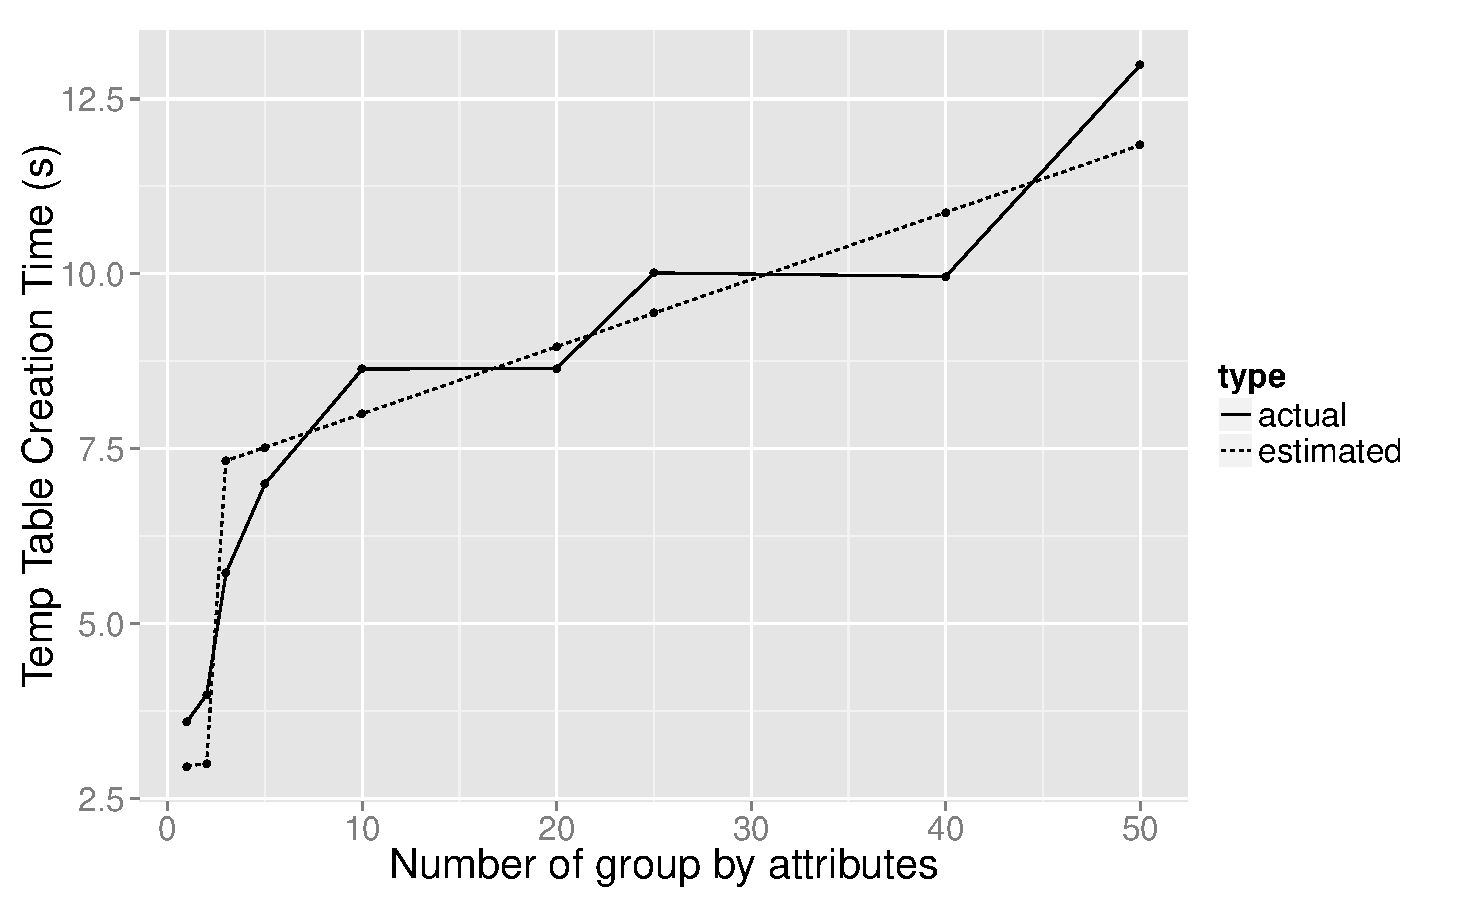
\includegraphics[width=6cm]{Images/create_time_fitted.pdf}
  \caption{Actual and Estimated Temp Table Query Time}
  \label{fig:create_time_fitted}
  
\end{figure}
\begin{figure}[h]
  \centering
    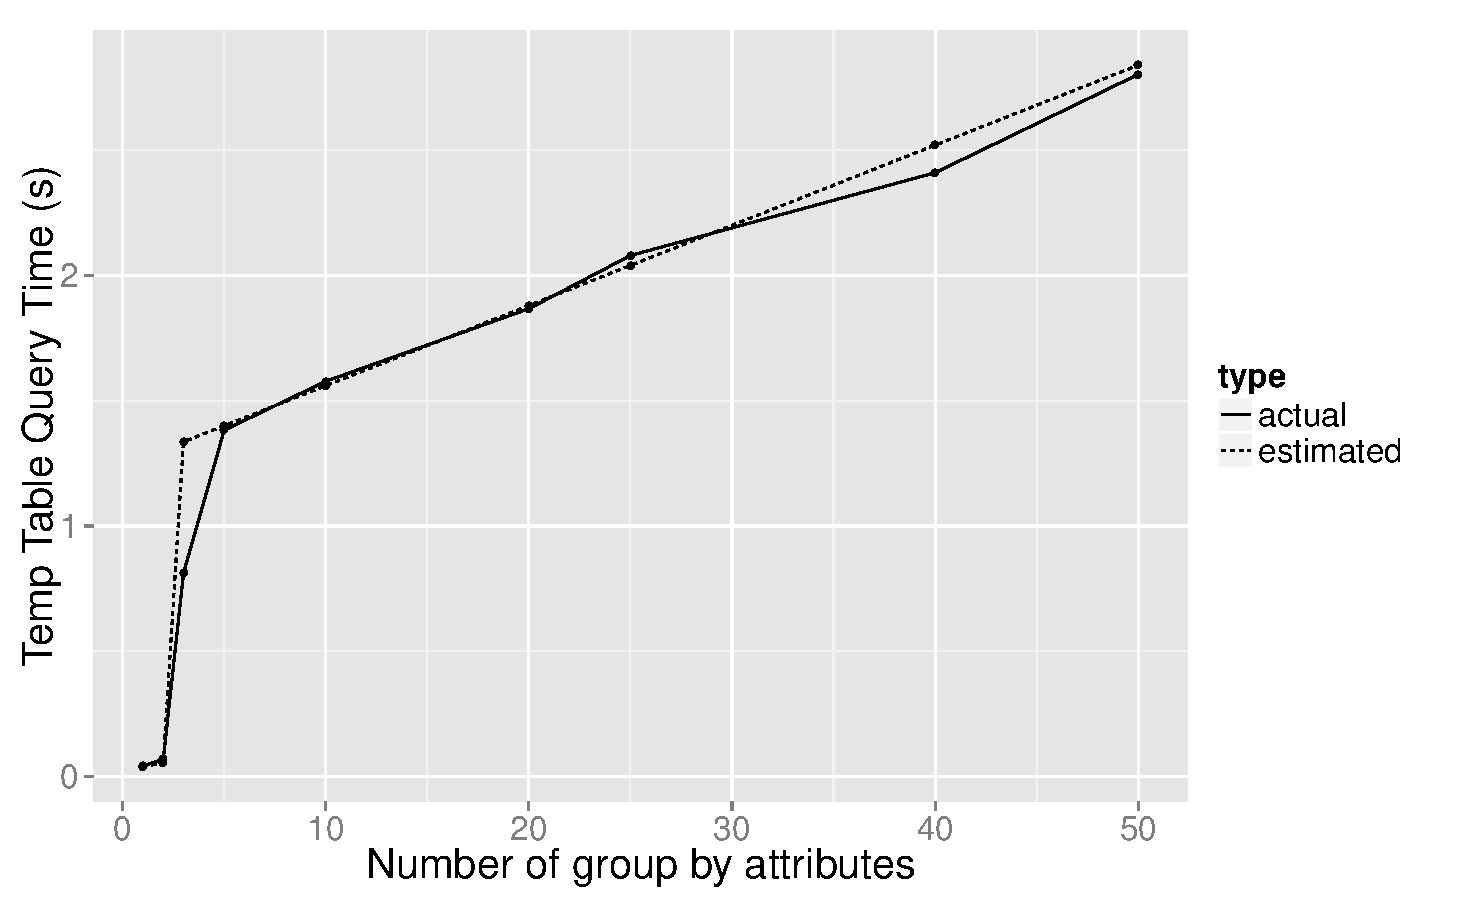
\includegraphics[width=6cm]{Images/query_time_fitted.pdf}
  \caption{Actual and Estimated Temp Table Query Time} 
  \label{fig:query_time_fitted}
\end{figure}

\begin{figure}[h]
  \centering
    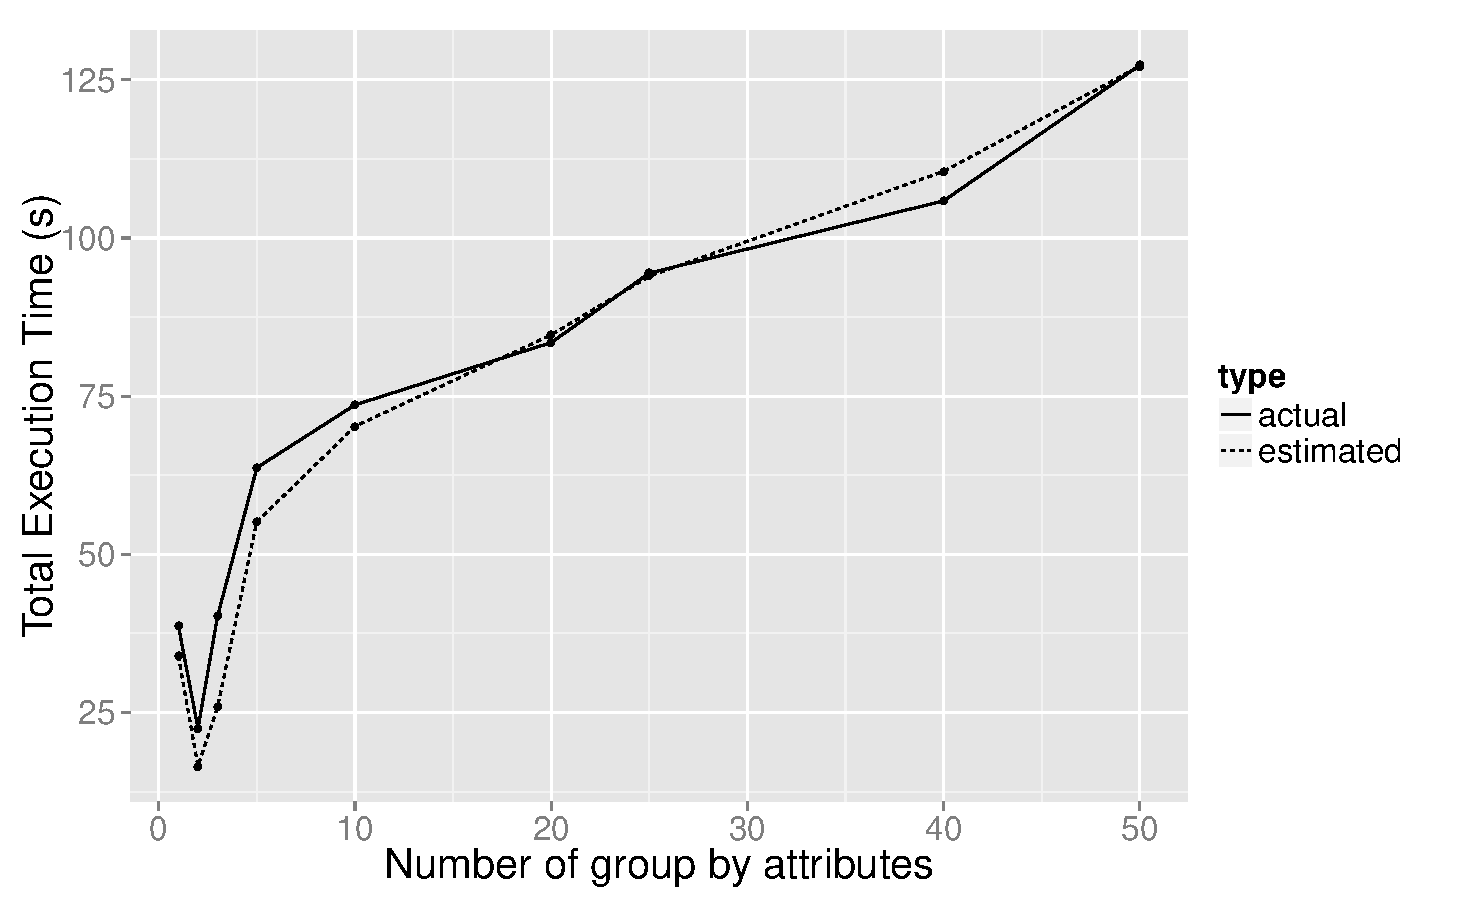
\includegraphics[width=6cm]{Images/total_time_fitted.pdf}
  \caption{Actual and Estimated Total Execution Time} 
    \label{fig:total_time_fitted}
\end{figure}

\subsection{Choosing \VizRecDB\ parameters based on the model}

{\bf Choosing Number of Parallel Queries:} The speed up offered by running
queries in parallel depends on the DBMS parameters such as maximum number of
connections, shared buffer size, etc. In our implementation, each phase of
processing can issue up to $n_{conn}$ queries in parallel, so in principle,
there may be up to $2 \ast n_{conn}$ queries running in parallel. Since each
DBMS has a maximum number of queries that can be executed in parallel,
$n_{conn}$ must be set to be smaller than half the maximum number of
connections. The exact number of connections will depend on the other workload
in the system and the size of the dataset. In our setup, $n_{conns}$=40 gives
the best results for a range of dataset sizes and system parameters.

{\bf Choosing $n_{agg}$:} Combining multiple aggregates offers a performance
gain that is almost linear in the number of aggregates, without any significant
penalty. As a result, we set $n_{agg}$ equal to the number of measure attributes
in the table.

{\bf Choosing dimension attributes to combined processing:}  As discussed in
Section \ref{subsec:mult_gb_expt}, the optimal number of distinct groups
consistently falls in the range 10,000 to 100,000. As a result, we set
$n_{groups}$, the maximum number of groups that any query can generate, to
100,000.
This parameter is used to pick dimension attributes that will be combined into a
single view query. For a set of attributes $a_1$\ldots$a_n$, the maximum number
of distinct groups that can be generated is $\prod_i a_i$. This is the worst
case bound since correlation between two attributes can only decrease the number
of distinct groups. \VizRecDB\ models the problem of grouping attributes with a
constraint on number of groups as a variant of bin-packing.
Specifically, \VizRecDB\ adopts the following problem formulation.

Let $n_{d_{i}}$ be the number of distinct values for dimension attribute $d_i$.
The traditional definition for bin packing states that given bins of size $V$
and $n$ items with size $a_1$\ldots$a_n$, find the minimum integer number of
bins and a corresponding partition of the set of items such that $\sum_{j} a_j$
$\leq$ $V$ for all $a_j$ belong to any given partition. In our setting, there is
a limit on the {\it product} (as opposed to the sum) of the sizes of items. As a
result, we formulate the problem as follows: Given bins (queries) of size $V$
($V$=100,000) and $d$ attributes with sizes $log(n_{d_{i}})$, find
the minimum number of bins and a corresponding partition of the $d$ attributes
such that $\sum_{j} log(n_{d_{j}})$, i.e. $\prod_{j} n_{d_{i}}$, $\leq$ $V$.
Bin-packing has been well studied and we use off-the-shelf software
\cite{glpk} to perform bin-packing on the dimension attributes.

\subsubsection{Experimental Evaluation with All Optimizations}

We now show performance results for \VizRecDB\ using the optimal parameter settings
described above. Specifically, we set $n_{conns}$=40, $n_{agg}$=$m$ (i.e.
number of measure attributes) and $n_{groups}$=100,000 for bin-packing. Further,
we apply the optimization of combinging target and comparison queries for each view. From
Figure \ref{fig:total_speed_up}, we see that the combination of all
optimizations gives us a speedup of about 100X for the Medium and Large
datasets (note the log scale on Y axis). Although the impact of optimizations is
relatively small for the Small dataset, we still observe that the total
execution time is halved. We thus see that the all the optimizations
taken together can enable \VizRecDB\ to run at near-interactive response times.

\begin{figure}[h]
  \centering
    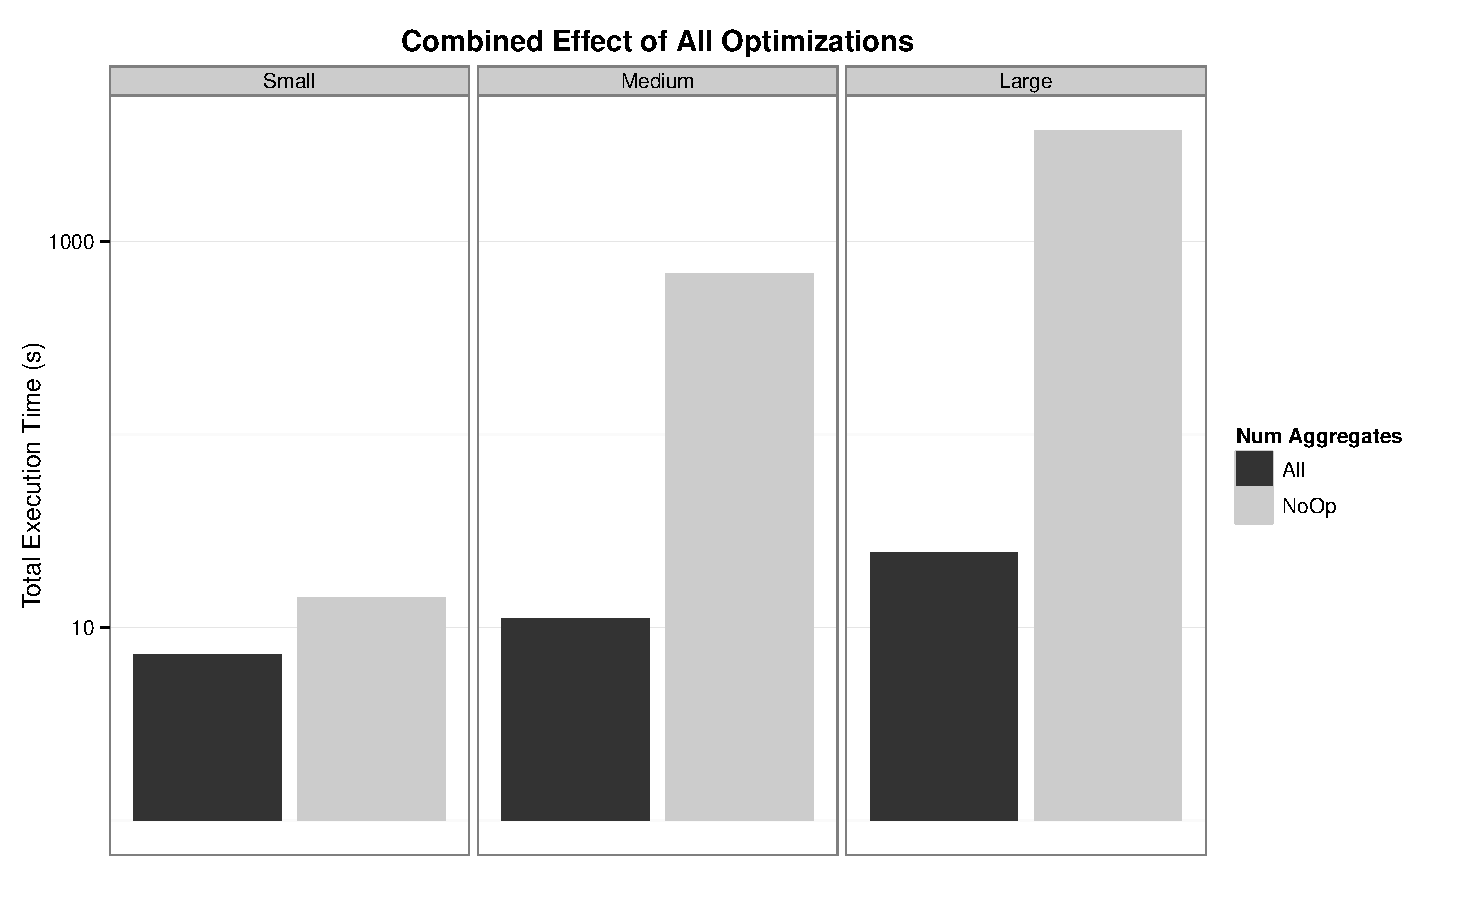
\includegraphics[width=6cm]{Images/total_speedup.pdf}
  \caption{Performance Speedup With Optimizations} 
  \label{fig:total_speed_up}
\end{figure}

\subsection{Main Memory Execution Engine}

We next describe performance characteristics of our main memory implementation
and the effect of our heuristics on performance and result accuracy.

\subsubsection{Effect of Confidence Interval based Pruning}

\subsubsection{Effect of MAB Pruning}

\subsection{DBMS vs. Main Memory Execution Engine}

\subsection{End-to-End Testing with Real Datasets}

\vspace{-2mm}
{\scriptsize
\bibliographystyle{abbrv}
\bibliography{visubib}
}
\end{document}